\chapter{Theoretical considerations}
\label{sec:2}

\section{Introduction}
\label{sec:2.1}  
Modern corpus linguistics (CL) as we understand it today arose during the 1960s, in the early days of the digital age. The appearance of electronic corpora in linguistics opened up the way for the development of numerous corpus-related sub-disciplines of linguistics. In the early 1990s, the use of corpora to study translational behavior was fully acknowledged within translation studies thanks to a seminal paper by Mona \citet{baker_corpus_1993}, and the sub-discipline of corpus-based translation studies (CBTS) was born. It is within this paradigm that this work is situated.

In the first part of this chapter (\sectref{sec:2.2}), I will introduce the discipline of CBTS. As will appear from this section, CBTS does not offer a clear-cut methodological framework to conduct a corpus-based study of meaning relationships in translation. The theoretical, methodological and descriptive footing to develop such a method will therefore be sought within other corpus-related areas of linguistics.

In \sectref{sec:2.3}, I will investigate a number of contrastive corpus studies. I will explore the notion of back-translation, a procedure which relies on translation equivalence and is known to reveal semantic relationships. Special attention will be given to the Semantic Mirrors Method (SMM), which exploits the procedure of back-translation and fulfills the prerequisites to validly compare meaning relationships in translated and non-translated language.

Various sub-disciplines of corpus semantics further provide useful insights for the investigation of semantic relationships in translation. In \sectref{sec:2.4.1}, I will elaborate on the notion of translational equivalence. Its operationalization within Word Sense Disambiguation (WSD) can be transferred to a corpus-based translational study as a solution to the operationalizability problem of equivalence. Corpus-based quantitative studies typically generate large amounts of data. In order to reveal the semantic information hidden in the corpus data, I choose to create bottom-up, statistical visualizations of semantic fields in translated and non-translated language. In \sectref{sec:2.4.2}, it will be shown that statistical visualizations of ``that what cannot be seen by the bare eye'' can be a potentially good lead towards meaningful representations of meaning relationships. In \sectref{sec:2.4.3}, I propose to combine the corpus-based quantitative visualizations with a theoretical framework from cognitive linguistics. I will propose to use the prototype model of category structure as a necessary basis for a coherent interpretation of the statistical visualizations.

\section{Corpus-based translation studies}
\label{sec:2.2}
In the first part of this section (\sectref{sec:2.2.1}), I will zoom in on the different types of corpora, which constitute the main methodological tool in CBTS. In the second part (\sectref{sec:2.2.2}), I will focus on precisely how this new sub-discipline arose within translation studies, by further exploring the research program set up by Baker. I will give extensive consideration to the translation universals paradigm and I will show why, in my opinion, research into universals on the semantic level has barely had any uptake within CBTS.\footnote{Admittedly, there exists research in CBTS that focuses on alternate subjects such as individual variation, translation norms and conventions or translation language change \citep[21]{zanettin_corpus_2013}. I choose, however, to focus on the universals research program which has undeniably dominated the field since the 1990s.} In addition, I will determine which universals seem best suited for the investigation of semantic relationships in translation. In \sectref{sec:2.2.3}, I will focus on the so-called cognitive turn in translation studies, which enabled the re-introduction of linguistic meaning into translation studies. The central notion of equivalence will be discussed in \sectref{sec:2.2.4}.\hypertarget{Corpora}{}

\subsection{Corpora}
\label{sec:2.2.1}  
Corpora come in so many flavors, shapes and sizes that it is virtually impossible to give an exhaustive overview of the existing corpora today \citep{mcenery_corpus_2012}. For learner corpora only, the Center for English Corpus Linguistics of the Université Catholique de Louvain lists close to 150 different corpora \citep{hiligsmann_learner_2015}. In an attempt to structure the vast number of corpora that is out there, several researchers have come up with corpus typologies; e.g \citet{johansson_role_1998} set out a typology for cross-linguistic research, \citet{baker_corpora_1995} and \citet{laviosa_corpus-based_2002} drew up typologies from the viewpoint of CBTS, \citet{brown_corpora_2006}, \citet{mccarthy_what_2010} and many others attempted to create typologies for the general purpose of corpus linguistics (CL), while numerous other overviews keep appearing in an effort to keep up with the unceasingly growing number of corpora.

Instead of undertaking a (necessarily non-exhaustive) overview of existing corpora, I will lay out the different dimensions along which a corpus can be defined: size, content and corpus languages. A better understanding of these dimensions is indispensable for the selection of a corpus that suits one’s research needs.

\subsubsection{Size}
\label{sec:2.2.1.1}  
The first electronic corpus – the Brown corpus – was established in 1961 and contained a little more than one million words. Ever since, the goal seems to be aimed at building ever larger corpora. It has indeed been remarked that some (rarer) linguistic phenomena could be absent from a corpus (and could consequently not be investigated) merely because the corpus was too small, so the idea that size mattered was quickly accepted. To overcome the obstacle of corpus size, the logical step was to ``simply'' build larger corpora: from a little more than 1 million words in 1961, to the appearance of the Oxford English corpus at the turn of the millennium counting over 2 billion words. By that time, the World Wide Web had started to be used as a corpus, too. Over the last decades, the average size of corpora has been growing steadily, with nowadays corpora on average containing hundreds of millions of words. However, this trend is observed to a far lesser extent regarding corpora in languages other than English, and even less so regarding bilingual or multilingual corpora. Corpora specifically suited for the study of translation, such as The English-Norwegian Parallel corpus – around 2.6 million words -- \citep{johansson_role_1998}, The Dutch Parallel corpus -- around 10 million words -- \citep{macken_dutch_2011} or the CroCo corpus – about 1 million words -- \citep{hansen-schirra_towards_2012} do not generally exceed 10 million words (see also the overview by \citealt[26--27]{zanettin_corpus_2013}). Although larger corpora would have the same advantages mentioned earlier with respect to the (monolingual) English corpora – more data allow the investigation of rarer linguistic phenomena that might remain unnoticed if the corpus size is too small – researchers in TS often have to content themselves with smaller corpora such as the ones cited above, simply because the bigger corpora that exist cannot be used for investigations in translation studies (comparable corpora have nevertheless been frequently used in CBTS).

\subsubsection{Content}
While for most of the history of CL, definitions of a corpus most often limited its content to text files, the recent appearance of multimodal corpora has introduced other types of data-carriers such as video and (live) streaming into the corpus world. Although this new development is uncontestably a very interesting one, I will not further explore this type of corpora (since this study will be carried out with a corpus consisting of text files).

A great deal of dimensions with respect to the types of text files that a corpus contains needs to be defined. First, the text files can consist of written material or they can contain transcriptions of spoken language, or both. Second, the corpus can aim to be representative of the general language; alternatively, it can contain different text types (the corpus can be balanced with respect to the different text types – or not), or it can be a specialized corpus, focusing on one particular text type (e.g. a corpus of legal texts). Thirdly, the corpus can be built up by complete texts or samples of texts (n words from the i\textsuperscript{th} to the j\textsuperscript{th} word of each text). The advantage of sampling is that “the number of words from each text can be exactly matched”, making it easier for the corpus designer to arrive at equal proportions per text type \citep[77]{deignan_metaphor_2005}. The danger with sampling is that some linguistic phenomena that tend to appear at the beginning or ending of texts might not be present in a corpus built up by samples (\citealt[77]{deignan_metaphor_2005}, referring to \citealt{stubbs_text_1996}). A corpus can also be a mix of samples and full texts, of course. The fourth dimension concerns the dynamic (open) versus static (closed) nature of a corpus: a closed corpus is delivered as a finite product, to which no texts are further added. A dynamic, open corpus on the other hand – also called a monitor corpus – is not so finite in the sense that materials can be added over time \citep[6]{mcenery_corpus_2012}. Both open and closed corpora can be employed for diachronic studies (of change over time) or synchronic studies (focusing on a particular period), all depending on how the corpus is used by the researcher \citep[3]{johansson_role_1998}.

\subsubsection{Languages of the corpus}
\label{sec:2.2.1.3}  
The final dimension concerns the number of languages present in a corpus. If there is only one language represented, the corpus is a monolingual one, with two languages, it is called bilingual, and with more than two languages present in the corpus, it is a multilingual corpus. \citet[36--38]{laviosa_corpus-based_2002} has proposed a further subdivision of these three types, which is presented below. Her corpus typology focuses on the applicability of corpora to the study of translation. Given the focus of this book on translated and non-translated language, I will maintain Laviosa’s typology:

\begin{itemize}
\item 
A \textsc{monolingual corpus} can be a single monolingual corpus, consisting of one set of texts (either translated texts or non-translated texts), in one language, whereas a comparable monolingual corpus consists of two monolingual corpora, one with translated and the other one with non-translated texts (all other design criteria are stable).
\item 
A \textsc{bilingual corpus} can be a comparable bilingual corpus, consisting of two monolingual corpora in two different languages – all other design criteria are or should be (as) stable (as possible) – that can consequently be compared to each other. A parallel bilingual corpus then consists of texts in two different languages, with the texts in one language being the originals of the translations in the other language. Parallel bilingual corpora can further be mono- or bi-directional. Mono-directionality means that language A is always the source language and language B always the target language; bi-directionality implies that language A and language B can both be source and target language.
\item 
A \textsc{comparable multilingual corpus} is similar to a comparable bilingual corpus, but with more than two languages involved; a parallel multilingual corpus is similar to a parallel bilingual corpus, again with the only difference being the number of languages involved. Laviosa indicates a supplementary difficulty here: parallel multilingual corpora can be mono-source – only one of the several languages is the source language, the other languages are target languages; bi-source – two of the several languages can be the source language; or multi-source – several or all of the languages in the corpus can serve as source language.
\end{itemize}

Laviosa established this corpus typology because she considered it to be “an essential step towards developing a coherent methodology in corpus-based translation studies” \citep[38]{laviosa_corpus-based_2002}.

\subsubsection{General issues with corpora}
\label{sec:2.2.1.4}  
The use of corpora in linguistics – although widespread and well-accepted in present-day linguistics – also raises a number of issues. One of the most common discussions in CL was initiated by \citet{tognini-bonelli_corpus_2001} and is concerned with the difference between cor\-pus-based and corpus-driven research. Put shortly, corpus-based approaches consider corpora as a method of research, whereas cor\-pus-driven approaches see corpora as the impetus for theoretical development in linguistics (for discussions on this topic, see \citealt[384--385]{hardie_two_2010}; \citealt[150 ff.]{mcenery_corpus_2012}). The importance of this distinction has been questioned by \citet[994]{ludeling_theory-driven_2009}, who finds the “sharp distinction” between corpus-based and corpus-driven approaches “overstated” and \citet[328]{gries_behavioral_2010}, who see no reason to consider CL a theory, but consider it a methodological paradigm.

A second issue concerns the representativeness, which is one of the most cited conditions imposed upon a corpus. This representative function can stretch from standard varieties of a language “to any kind of specialized language (represented in a domain-specific corpus)” \citep[11]{aijmer_state_1991}. However, no corpus – irrespective of how careful the compilation process has been carried out – can ever claim absolute representativeness. For instance, corpora that do not explicitly claim text-genre balancedness are sometimes only representative of the journalistic text type, because this is the text type that is most easily available. Even for an (explicitly) text-type balanced corpus, one can never be sure whose language the corpus is representative of. As Deignan puts it clearly:

\begin{quote}
Because there is such a wide variation in the range and relative proportions of text types that we each see and hear, no corpus could ever represent anyone’s personal experience of language more than fleetingly. This does not have to be seen as a disadvantage; it can be argued that a well-balanced corpus is superior to an individual’s personal corpus in its range and balance \citep[91]{deignan_metaphor_2005}.
\end{quote}

The importance of representativeness is also related to the type of research one wishes to conduct: it is important for a semanticist looking for the many meanings of, for instance, the lexeme \textit{translation} to have a corpus at one’s disposal that is representative of different text types so as to detect the different (metaphorical) meanings this lexeme is likely to have in different genres. Overall, if we let go of the illusive idea of absolute representativeness, and provided one compiles or selects their corpus with caution, then a corpus built in a balanced way with respect to different text types and compiled of texts selected from a wide range of different sources can be held as the current best possible representation of a standard variety of a language.

Finally, a third issue focuses on the advantages and disadvantages of parallel corpora. Whereas parallel corpora consist of source texts and their translations, the texts in a comparable corpus are simply comparable to each other according to a number of parameters set by the corpus designer (e.g. text length, genre, etc.) but they are not each other’s translational counterparts. The issue of comparability is the weak point of comparable corpora since “[s]ome types of text are culture-specific and simply have no exact equivalent in other languages” \citep[19]{granger_corpus_2003}. On a micro-textual level, it may be difficult to know which forms in the compared languages of the comparable corpus have similar meanings and pragmatic functions, and consequently, which forms can be compared and which ones cannot \citep[5]{johansson_translational_1998}. On the other hand, comparable corpora seem to be easier and faster to compile than parallel corpora, since it is usually more straightforward to identify texts as original texts or as translations than it is to find source texts with their matching translations. A drawback of parallel corpora, however, is that all texts labeled as \textit{original\slash non-translated} in a parallel corpus (representing for instance the native, standard variety of a language) have at some point been selected to be translated (since all non-translated texts in a parallel corpus are a source language text of a translated text in the corpus). This does not alter anything to the ``originality'' of the original language of course, but it should be kept in mind that the presence of texts in a parallel corpus can be based on their ``suitability'' to be translated (and hence, their absence can be based on their unsuitability). In order to overcome this problem, it is possible to include a monolingual reference corpus for supplementary comparison, but studies that have done so faced comparability issues due to corpus size or due to the uncertainty about the (translational) status of the texts in the presumed original language corpora (see e.g.: \citealt{musolff_conceptual_2014}).

\subsection{Baker’s universals}\ia{Baker, Mona@Baker, Mona|(}
\label{sec:2.2.2}  
\hypertarget{Bakersuniversals}{}
The paper that has literally catapulted translation studies into the era of corpus research – although preceded by work by \citet{toury_search_1980}, \citet{wollin_translationese_1986} and Frawley’s idea of third code \citep{frawley_translation:_1984} – was without a doubt Mona Baker’s 1993 seminal article \textit{Corpus Linguistics and Translation Studies}. Baker indeed foresaw that:

\begin{quote}
the techniques and methodology developed in the field of corpus linguistics will have a direct impact on the emerging discipline of translation studies, particularly with respect to its theoretical and descriptive branches \citep[233]{baker_corpus_1993}.
\end{quote}

The article provoked a true corpus turn in translation studies leading to the development of a research program that was mainly constructed on the basis of the idea of translation universals, equally proposed in that same article. But why was this corpus turn so much needed in translation studies? The main reason was probably that the positing of this new paradigm within TS allowed for an emancipation of the discipline with respect to other adjacent linguistic disciplines and especially with respect to contrastive linguistics, where translations were seen as a useful methodological tool rather than an object of study (see \sectref{sec:2.3}). Baker assigns a new and prominent role to parallel and in particular to comparable corpora: instead of dismissing translations as “second-hand and distorted versions of ``real'' texts” \citep[233]{baker_corpus_1993}, she puts them at the center of attention, claiming that the interest for TS is precisely to study in what way translations, as “genuine communicative events and as such [...] neither inferior nor superior to other communicative events in any language” \citep[234]{baker_corpus_1993} differ from non-translations. She asserts that a number of preparatory parameters needed to be set (e.g. the introduction of corpora in TS) so that this type of research could actually come into being:

\begin{quote}
There is now an urgent need to explore the potential for using large computerized corpora in translation studies. It seems to me that most of the components for realizing this potential are in place. The emphasis has shifted from meaning to usage, and the notion of equivalence is gradually giving way to that of norms. The status of the source text has been undermined and we have managed to make the leap from source-text-bound rules and imperatives to descriptive categories. There is increasing interest in features of translated texts per se and we are beginning to develop a descriptive branch of the discipline with well-defined objectives and an explicit program. [...] A suitable methodology and a set of very powerful and adaptable tools are now available from corpus linguistics \citep[248]{baker_corpus_1993}.
\end{quote}

Baker urges researchers to move on from a prescriptive to a descriptive branch of TS and to do so via the methodology and tools of CL. Instead of proposing or imposing rules on how one should translate or to prescribe what translation should be, TS needs to explore what translation is by investigating the actual usage in translation and by exploring the specific features of translated texts. In this respect, Baker sees the need of dismissing terms such as equivalence, correspondence and shifts “which betray a preoccupation with practical issues such as the training of translators” \citep[235]{baker_corpus_1993}. The fact that she can actually dismiss those terms has to do with another proposed attention shift: instead of focusing on the source text – which in Baker’s view is precisely the source of the rule-governedness and prescriptive nature of TS –, she proposes to focus on the target text, i.e. the translated texts themselves and their features. The dismissal of the terms equivalence, correspondence and shifts, is, however, only possible if one lets go of the contrastive outlook – and this was precisely Baker’s objective, an objective that has been put into practice in numerous studies comparing translated with non-translated language on the basis of comparable monolingual corpora (e.g. \citealt{laviosa_core_1998,olohan_reporting_2000,mutesayire_apposition_2004,xiao_how_2010} etc.). Although this attention shift towards the target text was a necessary step in the development of TS, voices claiming the inevitability of involving the source text into translational corpus research would quickly be heard too (see this volume). By the turn of the century, CBTS had established itself as a new paradigm within TS:

\begin{quote}
This new paradigm, corpus-based translation studies (CTS), can be defined as the branch of the discipline that uses corpora of original and\slash or translated text for the empirical study of the product and process of translation, the elaboration of theoretical constructs, and the training of translators. CTS makes use of a rigorous and flexible methodology, theoretical principles are firmly based on empirical observations, it uses both inductive and deductive approaches to the investigation of translation and translating, and it encourages dialogue and co-operation between theoretical, empirical, and applied researchers \citep[45]{granger_corpora_2003}.
\end{quote}

In that same 1993 seminal article, Mona Baker proposed a research program for CBTS, which has as its most important task to determine what distinguishes translated text from non-translated text:

\begin{quote}
[I]t will be necessary to develop tools that will enable us to identify universal features of translation, that is features which typically occur in translated text rather than original utterances and which are not the result of interference from specific linguistic systems \citep[243]{baker_corpus_1993}.
\end{quote}

Although Baker initially proposed six different types of universals (\citeyear[243--245]{baker_corpus_1993}), I will give an overview here of the four universals as presented by Baker in her \citeyear{baker_corpus-based_1996} article \textit{Corpus-based translation studies: The challenges that lie ahead}. This latter list of four universals – each of which are now properly named, unlike the list of six universals in the 1993 article – has indeed been taken as a standard reference to Baker’s universals (with only occasional references to the sometimes more vague terms used in the 1993 article). The establishment of this list is “[b]ased on small-scale studies and casual observation” \citep[243]{baker_corpus_1993}, but by virtue of corpus research, Baker hopes to find evidence for the existence or absence of these presumed universals.

\subsubsection{Explicitation}
\label{sec:2.2.2.1}  
Before Baker posited explicitation as one of the presumed features of translated language, \citet{house_shifts_1986} had already proposed the Explicitation Hypothesis, claiming that explicitation was “a universal strategy inherent in the process of language mediation” \citep[21]{house_shifts_1986}. Applied to TS, it then became “inherent in the process of translation”, since translation could be considered one of the ultimate forms of language mediation. Baker, following Blum-Kulka, defined explicitation as follows:

\begin{quote}
I take “explicitation” to mean that there is an overall tendency to spell things out rather than leave them implicit in translation \citep[180]{baker_corpus-based_1996}.
\end{quote}

Explicitation may consequently be determined by looking at text length (if it is true that things are overall more spelt out in translation, this should lead to an increased text length); or may manifest itself via syntactic or lexical devices. Numerous studies were carried out to test the Explicitation Hypothesis, e.g. \citet{overas_search_1998}, \citet{olohan_reporting_2000}, \citet{olohan_how_2003}, \citet{mutesayire_apposition_2004}, \citet{mauranen_explicitation_2004} and many others (see \citealt{Kruger2012} or \citealt{zanettin_corpus_2013} for overviews of the translation universals literature).

A study on syntactic explicitation, carried out by \citet{olohan_reporting_2000} focused on optional \textit{that} in reported speech and concluded that there was indeed an overall preference to use \textit{that} instead of the zero-connective in translated as opposed to original English (the study concentrated on forms of \textit{say} and \textit{tell)} \citep[157]{olohan_reporting_2000}. Although the evidence and argumentation in favor of this conclusion do seem convincing and are often cited as a confirmation of the Explicitation Hypothesis, \citet[10--11]{becher_abandoning_2010} argues that the observed increase of optional \textit{that} in translated language can be more plausibly explained as either source language interference or conservatism. As for source language interference, the increased use of \textit{that} may be explained as follows: some source languages may require \textit{that} in reported speech, other source languages may or may not allow it. The source language(s) (if they were known, which is not the case in Olohan and Baker’s study) could then explain the increased use of \textit{that} in the sense that the greater the number of source languages in the corpus which require \textit{that}, the more likely the increased number of \textit{that} in translated language is due to source language interference. The increased number of \textit{that} in translated language could also be attributed to translators’ alleged conservatism \citep{becher_abandoning_2010}. If Baker’s statements (\citealt[244]{baker_corpus_1993}, \citealt[183]{baker_corpus-based_1996}) that translators have more conservative linguistic habits than other text writers are to be taken as true, Becher argues that it would in fact quite straightforwardly (or at least more straightforwardly than the Explicitation Hypothesis) explain the increased use of optional \textit{that}, since this is the more ``conservative'' option in English (it cannot be left out after more formal and less common verbs).

Although Baker’s definition of explicitation seems quite unequivocal at first sight, and (quite) easy to identify contrastively on an individual sentence level, it is much more difficult to maintain it as a universal hypothesis and even more difficult when the implied source languages are unknown and cannot be taken into account. A phenomenon of zero-attestation vs.\ attestation may or may not be interpreted as explicitation, but, as \citet{becher_abandoning_2010} has shown, other hypotheses that “do not presuppose a subconscious tendency to explicitate on the part of translators” (\citeyear[11]{becher_abandoning_2010}) may easily overrule it. Becher, for that matter, also refutes Øverås’ (\citeyear{overas_search_1998}) arguments in favor of explicitation \citep[12--16]{becher_abandoning_2010}. He furthermore concludes that translators opt for explicitation on the basis of the same considerations as writers of original texts do and that there is consequently no such thing as translation-inherent explicitation \citep[22--23]{becher_abandoning_2010}.

\subsubsection{Simplification}
\label{sec:2.2.2.2}  
\begin{quote}
We can tentatively define “simplification” as the tendency to simplify the language used in translation \citep[181]{baker_corpus-based_1996}.
\end{quote}

With regard to the operationalization of simplification in a corpus study, Baker suggests that “[t]ranslators [...] may be inclined to break up long sentences in translation, so we might look at average sentence length in both source vs.\ target texts [...]” \citep[181]{baker_corpus-based_1996}. \citet{thelen_comparable_1996} carried out such a study and found that average sentence length in translated texts was significantly lower than average sentence length in a corpus of non-translated texts \citep[181]{baker_corpus-based_1996}. However, the argument that shorter average sentences are “simpler” than longer sentences is a (mere) intuition about how texts can be “simplified”. In research related to second language acquisition, it has been shown that coherence markers increase text comprehension more than fragmentation (the use of shorter sentences) does \citep{land_zwakke_2009}. So, even if it were true that the average sentence length in translated texts is shorter than in non-translated texts, and even if the translators did produce shorter sentences out of a primary concern with the comprehensibility of their text, this does not mean that the text does de facto become simpler. Although “simplification involves making things easier for the reader” \citep[182]{baker_corpus-based_1996}, conscious acts to do so may well have a contrary effect. Baker adds that, although simplification does not necessarily mean that the text is rendered more explicitly, “it does tend to involve also selecting an interpretation and blocking other interpretations, and in this sense raises the level of explicitness by resolving ambiguity” \citep[182]{baker_corpus-based_1996}. An act of simplification may thus be realized via an explicitation in the text, which makes it obviously extremely hard for the TS researcher to distinguish explicitation from simplification.

Another way of operationalizing simplification is via indicators such as lexical variety or lexical density. Lexical variety (also called lexical diversity or vocabulary range) can be accessed via the calculation of the type-token ratio – the number of unique word types per total number of (or usually per thousand) tokens. The closer the type-token ratio is to 1 (or 100\%), the more varied the vocabulary in a given text or corpus is (see e.g. \citealt{laviosa_core_1998}). Lexical density (information load) is “the percentage of lexical as opposed to grammatical items in a given text or corpus of texts” \citep[237]{baker_corpora_1995}. Different text types can, however, show different levels of lexical density, so that the measure can only be used for intra-text type comparison in TS. Alternatively, lexical density can be measured by calculating mean word length \citep{Kruger2012}. The use of this measure is based on the assumption that “word length can be seen as a measure of morphological complexity. [...] [M]ean word length is also an indicator of lexical specificity. Shorter words are more frequent and more general, while longer words are less frequent and more specific” \citep[366]{Kruger2012}.

The measures proposed to investigate simplification on the level of a text or (part of) a corpus are mainly quantitative and very little or no doubt can arise as to how a type-token ratio or a mean word length should be operationalized. However, one might wonder to what extent these measures really indicate simplification in Baker’s sense of “making things easier for the reader” \citep[182]{baker_corpus-based_1996}. Some of the measures discussed here such as average sentence length do not seem to “make things easier” \citep{baker_corpus-based_1996} at all. In addition, from the viewpoint of readability research, which is equally concerned with “what makes some texts easier to read than others” (\citealt{dubay_principles_2004}; cited by \citealt{clercq_using_2014}), the measures for simplification in translated texts do not suffice (any longer). Although traditional readability formulas do or did indeed use the kind of measures proposed above as measures of simplification, readability research has evolved rapidly over the last decade or so:

\begin{quote}
In recent studies, readability has been linked with more complex lexical and syntactic text characteristics [...] and more recently, discourse features capturing local and global coherence across text are also being scrutinized [...] \citep[294]{clercq_using_2014}.
\end{quote}\largerpage

As a consequence, a more up-to-date and complete measure of simplification in TS would necessarily have to take into account advances made in readability research before any statements could be made as to the overall simplification of a text or corpus under study. Although readability measures were used to assess the difficulty of the source text of a translation task \citep{gopferich_indicators_2009,sun_measuring_2014}, measures of readability have – to my knowledge – not yet been used to test this translation universal but could give researchers firmer quantitative ground to stand on in the comparison of translated and non-translated texts. Finally, if one is indeed interested in discovering whether translated texts are \textit{easier} \textit{to} \textit{understand} than non-translated texts, the question whether they are \textit{simpler} might just be the wrong question. Rather, researchers in TS could ask themselves: do we see that factors commonly known to raise readability equally appear in translated texts?

\subsubsection{Normalization/conservatism}\largerpage
\label{sec:2.2.2.3}  
\begin{quote}
“Normalisation” (or “conservatism”) is a tendency to exaggerate features of the target language and to conform to its typical patterns. This tendency is quite possibly influenced by the status of the source text and the source language, so that the higher the status of the source text and language, the less the tendency to normalise \citep[183]{baker_corpus-based_1996}.
\end{quote}

The third universal feature of translation, normalization – also referred to as \textit{conventionalization}, \textit{standardization} or \textit{sanitization} \citep[23]{zanettin_corpus_2013} – is defined as a tendency to conform with typical features of the target language, and will depend on the status of the source language: a higher status of the source language will decrease the tendency to normalize. By virtue of its own definition, normalization then in fact dismisses itself as a universal strictu sensu: if normalization is susceptible to the status of the source language, it cannot be universal anymore, since universals are by definition “not the result of interference from specific linguistic systems” (cf. the quote by Baker in \sectref{sec:2.2.2}). Despite Baker’s own concession to the strict interpretation of universals, source-language related phenomena such as interference have often been excluded from the universals research paradigm, under the pretext of posing “serious problems for any kind of causal explanation of the findings” \citep[311]{pym_tourys_2008}. This being said, normalization in translation has been widely researched via apparent operators such as hapax legomena as a feature of the lexical creativity \citep{kenny_lexis_2001}, typical grammatical features \citep{kranich_between_2011} and degrees of formality of pairs of near synonyms  \citep{oakes_lexical_2012}. The results of these studies are, however, far from unequivocal in stating that normalization is usual business in translation. \citet[210]{kenny_lexis_2001} concludes that “lexical normalization has been found, but it is far from an automatic response to lexical creativity in source texts” and \citet[338]{oakes_lexical_2012} conclude (i) that degrees of formality in translated texts may differ depending on the source text, (ii) that translated texts are not always more formal (more conservative) than non-translated texts and (iii) that, when translating into the same target language, translators normalize less when translating from one source language and more when translating from another source.

As Baker intuited about normalization, it seems very hard to pretend that normalizing trends in translated texts are (completely) source language independent. As a consequence, source language influence on translated texts has been taken into account with regards to the normalization hypothesis, and researchers like Teich have hypothesized a two-directional influence on translated texts:

\begin{quote}
\begin{itemize} 
	\item translations are different from comparable texts in the same language because the \textit{source} \textit{language} \textit{shines} \textit{through}. How does the source language shine through in translations and how can this shining-through be described?
	\item translations are different from comparable texts in the same language because they try to be even more ``typical'', \textit{more} \textit{``normal''} of the target language than are original texts in the same language. In what terms can ``normal'' be defined and how can that definition be applied to translations?
\end{itemize}
\hfill(\citealt[61--62]{teich_cross-linguistic_2003}, my emphasis)
\end{quote}

While the second hypothesis corresponds to the classic definition of normalization (adherence to target language norms), the first one hypothesizes that normalization can also take place in the opposite direction (adherence to source language norms). In such cases, the source language is said to literally \textit{shine} \textit{through} in translated texts. \citet[136]{kranich_between_2011} puts forward the idea that the specific features of translated texts might well be the result of a “hybridization of normalization and shining through” where the specific features observed in translated texts would hold a balance between a tendency to conform to the norms of the target text and a propensity to adopt features that are typical for the source language at hand.

\subsubsection{Levelling out}\largerpage
\label{sec:2.2.2.4}  
\begin{quote}
“[T]he tendency of translated text to gravitate towards the centre of a continuum” \citep[184]{baker_corpus-based_1996}.
\end{quote}

While the above definition might seem somewhat vague, the idea of \textit{levelling} \textit{out} means that “we can expect less variation among individual texts in a translation corpus than among those in a corpus of original texts” \citep[177]{baker_corpus-based_1996}. Translated texts would thus be more alike amongst each other than non-translated texts. Just like for simplification, the measures to investigate levelling out are lexical density and type-token ratio; the difference lies in the conclusions that are drawn from these measures. From the point of view of simplification, a lower lexical density in translation leads to the conclusion that translated texts are simpler than original texts. From the perspective of levelling out, the question is raised whether lexical density levels amongst translated texts are more similar than lexical density levels amongst non-translated texts. In other words, levelling out is investigated by comparing the variation of a certain feature (e.g. lexical density or type-token ratio) between translated and non-translated texts \citep[184]{baker_corpus-based_1996}. As Baker already indicated in 1996, levelling out is probably the universal that has received the least attention in the literature. Olohan’s 2004 overview of the state of the art in corpus studies in translation confirms that this universal is the one for which least empirical investigation has been set out as it seems to be the most difficult one to measure \citep[100]{Olohan2004}. Later overviews by \citet{Kruger2012} or \citet{zanettin_corpus_2013} show that the decade following Olohan’s overview has not brought much change to this. Kruger mentions the existence of the universal of levelling out but does not take it up in her overview of universals (most probably because there were no studies focusing on levelling out that could be discussed). She does indicate, with respect to her own study presented in the same article, that some evidence has been found for this universal “since register differences are largely neutralized in the translated subcorpus” \citep[369]{Kruger2012}. Zanettin mentions not one study investigating “linguistic indicators of leveling out or the way to implement them through computational operators” \citep[23]{zanettin_corpus_2013}.\largerpage

In short, although the idea behind the universal of levelling out is potentially interesting, to my knowledge, no studies have so far focused on this universal in particular. This is most probably because levelling out is often (mis)taken for the universal of simplification, a universal that is operationalizable ``on the surface'' of the corpus and does not require the use of statistical techniques -- which are needed if one wants to gain more insights into the levelling out of a certain feature. In order to arrive at an understanding of levelling out, one would indeed need to have an idea of an average range of a specific feature in translated texts and compare it to the average range of that same feature in original texts so as to understand whether translated texts are more like each other than non-translated texts. It is, in my opinion, precisely investigations into meaning in translation that would best ``suit'' this universal (which would consequently explain why this universal has never been properly investigated). Contrary to the other universals, a certain level of abstraction will therefore be needed (a common requirement for both the investigation of meaning as well as for the universal of levelling out).

\subsubsection{Universals: The more the merrier?}
\label{sec:2.2.2.5}  
Over the last more two and a half decades, the notion of translation universals has set many tongues wagging. In the mid-2000s, after ten years of universals research, claims of evidence for the existence of universals by some researchers, and statements by others that universals could simply not be investigated, had left the research community with the question whether universals did or did not exist at all \citep[1]{Mauranen2004}. Some universals were indeed refuted (see e.g. \citealt{becher_abandoning_2010}) and new ones, such as the Unique Items Hypothesis  \citep{mauranen_unique_2004} or the Asymmetry Hypothesis \citep{dimitriu_asymmetry_2009} were added to the list. The Unique Items Hypothesis states that some features that are unique to the target language will appear less or will not appear at all in translated language, because they are not triggered by any source language feature  (\citealt{mauranen_unique_2004}; see also \citealt{gambier_what_2004} for a revision of the hypothesis). The Asymmetry Hypothesis, first proposed by \citet{dimitriu_asymmetry_2009} and modified by \citet{becher_abandoning_2010}, affirms that “[o]bligatory, optional and pragmatic explicitations tend to be more frequent than the corresponding implicitations regardless of the SL\slash TL constellation at hand”. Although a universal ought to be a feature that appears irrespective of the source language, scholars quickly understood that – in order to figure out where certain phenomena were coming from – the inclusion of the source language seemed inevitable. However, the inclusion of the a priori excluded feature of source language within the universals paradigm as well as the expansive number of universals was not without consequences for the viability of the notion. 

Chesterman proposed to divide the (growing number of) universals into two categories, the S-universals (“characteristics of the way in which translators process the source text” \citealt[39]{gambier_what_2004} and T-universals (“characteristics of the way in which translators use the target language”, \citealt[39]{gambier_what_2004}). Chesterman’s S-universals are features such as lengthening (translated texts tend to be longer than their originals) – a feature of translated language that had been proposed by  \citet[185]{vinay_stylistique_1958} – and \citegen{toury_descriptive_1995} well-known laws of interference (source text features are transferred to the target text) and growing standardization (a source-text specific feature will be replaced by a more ``common'' expression in the target text), the latter having a lot in common with Baker’s definition of normalization. Amidst the potential T-universals, we find inter alia simplification and Tirkonnen-Condit’s Unique Items Hypothesis. Chesterman moreover counters the difficulty of testing the universals of translation within the scope of one study, by proposing what he calls “the low road”, where “a universal hypothesis might also be tentatively proposed on the basis of empirical results pertaining only to a subset. [...] [T]he criteria on which the subset is defined [...] [will] define the conditions that determine and limit the scope of the claim” \citep[40]{gambier_what_2004}. Following Chesterman, any of the generalizations made on the basis of a corpus study should indeed first and foremost apply to the language-pair(s), the period, the text genre(s) etc. which are selected by the researcher (and often determined by the chosen (sub-)corpus or by the parameters that were set for corpus creation). In order to make general, universal claims, the same study would have to be repeated for an as wide as possible variety of language pairs, as many periods and as many genres as possible. The apparent unfeasibility of doing the latter has led researchers such as Mauranen to dismiss the idea of universality at once, but to opt for \textit{general} \textit{tendencies} (\citeyear[35]{anderman_universal_2008}):

\begin{quote}
The term ``universals'' does not, then, necessarily refer only to absolute laws, which are true without exception. Rather, most of the suggested universal features are general or law-like tendencies, or high probabilities of occurrence \citep[35]{anderman_universal_2008}.
\end{quote}

It is precisely the claim of universality of the translation universals which has been bothering the research community interested in the subject. The newly added universals or revisions such as Chesterman’s S- and T-universals all seem to try to do away with this idea of universal applicability. Other scholars have introduced terms such as \textit{general} \textit{tendencies} of translation in an attempt to tone down or at least nuance the universality claim. Mauranen refers to the field of general linguistics, where the term \textit{universals} is also used, but where it has become general practice “to take into account different kinds of general tendencies shared by a large number of languages, not only ``absolute'' universals, that is, features shared by every human language” \citep[35]{anderman_universal_2008}, and she suggests that the term \textit{universals} should be defined in a similar way within TS.

As a result of this unceasing universals debate, it was realized that translational behavior is multidimensional in nature \citep{de_sutter_inevitability_2013}, and that, in addition to purely linguistic matters, there are also a number of social, cultural, ideological and cognitive constraints acting upon translation \citep{baker_role_1999}. In order to include these constraints into the research paradigm, alternative methodological approaches have recently been proposed. In translation process research, triangulation (the combination of several data gathering techniques and methodologies) has become increasingly common (see e.g. \citealt{alves_foreword._2003,carl_triangulating_2010,shreve_integrative_2010}). In addition, the use of multivariate statistics has recently been introduced into CBTS. “[M]ultivariate data are typically represented in a matrix form with rows holding the units and columns holding the variables” \citep[302]{meng_multivariate_2012}. By representing corpus data as (frequency) matrices, the complexity of the (type of) linguistic data in (corpus-based) translational research can be (more easily) tackled. These techniques “allow us to preserve the rich diversity of linguistic forms, while at the same time reducing the variation in a principled way to a simpler, more interpretable structure” \citep[301]{meng_multivariate_2012}. Recent studies by \citeauthor{delaere_is_2012} (\citeyear*{delaere_is_2012}), \citeauthor{szmrecsanyi_weakly_2014} (\citeyear*{szmrecsanyi_weakly_2014}) and the studies presented in the edited volumes by \citet{oakes_quantitative_2012} and \citet{DeSutterEtAl2017} have shown that multivariate statistical methods can be successfully implemented into CBTS. In this work, I will use multivariate statistical techniques to capture the complexity of the meaning relationships in translated and non-translated language by using translations as the variables of source-language lexemes (and vice-versa) in frequency matrices (this will be further explained in \sectref{sec:2.4} as well as in \chapref{sec:3}).

\subsubsection{The relationship between universals and meaning}
\label{sec:2.2.2.6}  
The impact of Baker’s 1993 article on the development of CBTS can hardly be overestimated. In \sectref{sec:2.2.2} I stated that Baker’s research program was both necessary and useful for the emancipation of CBTS and even for TS as a whole. However, some of Baker’s propositions have heavily determined the focal points of TS in the years to follow. For instance, Baker’s dismissal of the source language, in an attempt to put translation and translated language at the center of attention, has led to studies which completely left out any consideration regarding the source language (since the type of corpora that were favored – comparable corpora – did not include the source texts of the translations in the corpus). This probably also led to an increased number of comparable corpora (instead of parallel corpora) because precisely these type of corpora were thought to serve the needs of CBTS best, a phenomenon that in its turn led to more target language oriented research in TS.

A similar scenario might apply for the study of meaning in CBTS. By announcing “the decline of the semantic view of translation” \citep[237]{baker_corpus_1993}, Baker attempted to get rid of clichéd, simplistic ideas about translation (the idea that translation is a mere word-for-word or sentence-for-sentence contrastive operation), but in this way she also declined to some extent the further study of meaning in translation. In the same way as the concepts of \textit{equivalence}, \textit{correspondence} and \textit{shifts} were dismissed because they were thought to betray a preoccupation with practical issues in translation \citep[235]{baker_corpus_1993}, the (contrastive) study of meaning in translation was set aside because such a study would imply that the researcher was “still trying to justify them [translated texts] or dismiss them by reference to their originals” \citep[235]{baker_corpus_1993}. Baker’s assertions seem to have impacted CBTS in the sense that studies of meaning proper in CBTS are rather scarce, and concepts such as \textit{equivalence}, \textit{correspondence} and \textit{shifts} were absent (because considered unnecessary) from the investigations that claimed to fall under the scope of the research program. This does not mean that there are no studies at all within CBTS that address the problem of meaning. In \sectref{sec:2.2.3}, I will show that any CBTS study concerned with meaning will at some point be confronted with the concepts of \textit{equivalence} and \textit{correspondence} or will avoid to engage in research into universals of translation.

A second reason why research into meaning in translation might have been shoved aside is that meaning finds itself at the very core of what translation is: according to numerous scholars in the field, meaning is “the invariant of translation” \citep[82]{lewandowska-tomasczyk_specification_2010}. Indeed, “it seems to be firmly embedded in public opinion that in translation it is the meaning that has to remain unchanged” \citep[82]{lewandowska-tomasczyk_specification_2010}. It appears to be widely accepted that invariant meaning is conveyed via lexicalized expressions from one language to another through translation. However, if we question the invariability of the invariant, we somehow remove the firm ground on which a lot of research in translation has so far been built. Nevertheless, in order to know if it is true that meaning is the invariant of translation, one will necessarily have to engage into empirical research into meaning and meaning relationships in translation.

Finally, a third reason why meaning might not have received the attention it deserved in TS, is that meaning is an abstract notion and therefore difficult to capture. This might have discouraged TS scholars from taking up the subject. In the following \sectref{sec:2.2.3}, some important investigations of meaning in translation carried out over the last two decades will be highlighted.\ia{Baker, Mona@Baker, Mona|)}

\subsection{The cognitive turn in translation studies}\label{sec:2.2.3}  
\subsubsection{\textit{Translation and meaning} series}\label{sec:2.2.3.1}  
The ten parts of the \textit{Translation and meaning} series (each of the volumes contains the proceedings of an international duo-colloquium which is held every five years in Maastricht and Łódź, under the auspices of Marcel Thelen\ia{Thelen, Marcel@Thelen, Marcel} and Barbara Lewandowska-Tomaszczyk)\ia{Lewandowska-Tomaszczyk, Barbara@Lewandowska-Tomaszczyk, Barbara} cover an incredibly wide range of subjects. There does not seem to exist a single branch of TS which is excluded from the series: anything from corpus work to machine translation to dictionary compilation, the translation of literary and holy texts, terminology, translator and interpreter training is included. However, very few studies in the series take a linguistic viewpoint on meaning. Most of the papers fit the series’ subject because of the general acceptance that translation \textit{is} meaning, and that meaning is the invariant of translation, leading to the possibility of including virtually any branch of TS into the series. \citeauthor{thelen_comparable_1996}’s \textit{Comparable corpora: Towards a corpus linguistic methodology for the empirical study of translation} in the third part of the series (\citeyear{thelen_comparable_1996}) for instance – although uncontestably making an important contribution to the propagation of corpus research and the universals program in TS – does not at all engage with the question of meaning invariance in translation, but implicitly accepts it as a bottom line. Other studies, such as  \citegen{lewandowska-tomasczyk_word_1992} \textit{Word against text: Lexical semantics and translation theory} (in the second part of the series) express their interest in lexical semantic studies and the possible contributions linguistics can make to TS. Unfortunately, they do not consider the scholarly contributions lexical semantics could make to the discipline of TS but (only) explain how lexical semantics could be of help for the professional translator \citep[100]{lewandowska-tomasczyk_specification_2010}. The same applies for corpora: a number of studies in the \textit{Translation and meaning} series use corpora to investigate (linguistic) meaning. They often focus on the utility of such tools for translation teaching and translation quality assessment but do not address the idea of meaning invariance in translation as such (e.g. \citealt{thelen_equivalence_1997,thelen_corpus-based_2007,thelen_semantic_2008}). One of the few studies that actually does engage in the question of meaning invariance in translation is \citeauthor{thelen_norwegian-english_1996}'s \textit{Norwegian-English translation and the role of certain connectives} (\citeyear{thelen_norwegian-english_1996}) where connectives are classified according to semantic categories which are subsequently compared. Halverson concludes that connectives change their semantics in translation and in this way, her conclusions point in the direction of the possibility of meaning variation in translation.

\subsubsection{The re-introduction of meaning in translation studies}\label{sec:2.2.3.2}  
The corpus turn from the 1990s – which ensued from descriptive translation studies (hence: DTS) – was the necessary prerequisite for TS to become a discipline in its own right. According to \citet[41]{thelen_translation_2002}, there were two “leading recurrent themes” in translation theory in the 1990s: corpus research and cognitive approaches. Within the first current – corpus research – the so-called universals paradigm was quickly adopted by a large group of scholars. As for the second current, one would have expected an emphasis on linguistic meaning and the status of meaning in TS, parallel to cognitive linguistics \citep[41]{thelen_translation_2002}. However, the earliest attestations of a cognitive TS did not immediately show interest in a re-introduction of linguistic meaning (and equivalence) but rather focused on corpus-based empirical and experimental (process) research and introduced, for instance, think-aloud protocols (see e.g. the volume edited by \citealt{tirkkonen-condit_tapping_2000}) which equally benefited from the cognitive-translational setting. \citet{rojo_cognitive_2013} summarized what was happening on the intersection of cognitive linguistics and translation by the end of the 1990s as follows:

\begin{quote}
The relevance of cognitive linguistics for translation arises mainly from the “experiential” notion of meaning proposed by cognitivists, which abandons the traditional notion of referential truth and highlights the central role of human experience and understanding \citep[7]{rojo_cognitive_2013}.
\end{quote}

Although the above mentioned “notion of referential truth” was abandoned within most cognitively oriented studies of translation, a number of scholars did propose a “linguistic-cognitive orientation” \citep{house_towards_2013}. House makes a strong plea in favor of a “linguistic-cognitive orientation” in TS, since “translation is above all an activity involving language and its cognitive basis” \citep[47]{house_towards_2013}. In her opinion, TS scholars have been so pre-occupied uncovering and investigating all the “external social, cultural, personal, historical etc. factors impinging on translation ``from the outside''{”} that they have somewhat forgotten about what translation is made of ``from the inside'' \citep[47]{house_towards_2013}. She argues in addition that a cognitive-linguistic view on translation could counterbalance the wide focus on these external factors:

\begin{quote}
For balance, I think it is also necessary and insightful to describe and explain how strategies of comprehending, decision making and re-verbalization\linebreak come about in a translator’s bilingual mind” \citep[46]{house_towards_2013}.
\end{quote}

In the following paragraphs, I will highlight a number of studies which have specifically engaged with this linguistic-cognitive orientation on TS. This non-exhaustive overview focuses on those studies which in my opinion have provided important insights for the study of translation within a linguistic-cognitive framework, especially with regards to the status of meaning in translation or the impact of translation on meaning. Early attestations of this linguistic-cognitive orientation include \citet{tabakowska_cognitive_1993}, who introduced notions from Lang-\linebreak acker’s\ia{Langacker, Ronald@Langacker, Ronald} Cognitive Grammar in TS, and \citegen{kussmaul_training_1995} idea that foregrounding and suppression of semantic features could be useful when translating complex meanings \citep[8]{rojo_cognitive_2013}. Research by \citet{wilss_knowledge_1996} also pointed towards a cognitive-linguistic approach to meaning in the 1990s.

\citet{korning_zethsen_corpus-based_2008} proposes to use cognitive semantics “as a tool for researchers within translation studies (TS) who are particularly interested in revealing evaluative aspects of the units of meaning of source texts and their translations” (\citeyear[249]{korning_zethsen_corpus-based_2008}). She suggests that (translation) scholars “should aim at a description of prototypical features, inherent or contextual” rather than “attempting an exhaustive analysis of a lexeme” (\citeyear[251]{korning_zethsen_corpus-based_2008}). One of her key focus areas is semantic prosody, i.e. “the spreading of connotational colouring beyond single word boundaries” (\citealt[68]{partington_patterns_1998} in: \citealt[256]{korning_zethsen_corpus-based_2008}). She concludes that:

\begin{quote}
Semantic prosody is bound with time to influence our perception of the concept of equivalence. A likely hypothesis is that the traditional problem of ``false friends'' within translation is much more pervasive than assumed up till now. Presumably equivalent words may have developed differently in two languages and have in time been influenced by the company they have kept and thereby developed different prosodies \citep[258]{korning_zethsen_corpus-based_2008}.
\end{quote}

Korning Zethsen touches here upon a semantic matter that might well be pervasive in translation, but which needs advanced (corpus) methods to be revealed. Moreover, by putting a concept such as semantic prosody at the center of attention of translational research, not only does she re-introduce the concept of equivalence, she also questions the ``invariance'' of meaning in translation and shows how corpus-research accompanied by interpretation can be used to uncover the importance of such subtle issues as semantic prosody in translation.

\citet{lewandowska-tomasczyk_specification_2010} takes the point of view of translation universals to investigate lexical specification and generalization. Her contrastive view on translation\linebreak (translation as transfer) is in apparent opposition with the mainstream research into universals, which generally refutes the contrastive concepts of equivalence and correspondence. Klaudy shows that the introduction of an equivalence-like concept (although a narrow one in comparison to what most translation studies scholars would understand as equivalence) makes it possible to study universals in a contrastive setting. She introduces the concept of \textit{lexical} \textit{transfer} \textit{operations}:

\begin{quote}
In our interpretation, “lexical transfer operations” is a collective term for all the systemic and routine-like operative moves developed by generations of translators to handle the difficulties stemming from the different lexical system and cultural context of the two languages functioning together in the process of translation \citep[81]{lewandowska-tomasczyk_specification_2010}.
\end{quote}

The identification of these “operative moves” can provide additional information on language differences not yet distinguished by contrastive lexicographers and bilingual dictionary builders. Klaudy furthermore expresses a special interest in the impact of the process of translation on systemic language differences (\citeyear[82]{lewandowska-tomasczyk_specification_2010}) and questions the “firmly embedded idea that meaning remains unchanged in translation” (\citeyear[82]{lewandowska-tomasczyk_specification_2010}). Klaudy makes a distinction between \textit{meaning} and \textit{sense} to explain the processing of meaning in translation. \textit{Meaning} covers “the criteria for the usage of a linguistic sign within a given language” and \textit{sense} “the relationship between the linguistic sign and a certain segment of reality (objects, events, persons, phenomena) here and now” \citep[83]{lewandowska-tomasczyk_specification_2010}. The process of translation involves the recreation of \textit{sense} in the TL, “instead of retaining the SL meaning” (\citeyear[83]{lewandowska-tomasczyk_specification_2010}). Klaudy sees the fact that translators “try to relate TL signs to reality according to SL rules of usage” as a frequent source of translation errors \citep[83]{lewandowska-tomasczyk_specification_2010}, and this is where according to Klaudy, meaning (in)variance ties up with translation universals.

In the volume edited by Rojo and Ibarretxe-Antuñano, \citet{rojo_who_2013} explores how cognitive models of meaning can be of use for translation. “Different cognitive approaches provide different visions of meaning, and they also lead to different theoretical frameworks for empirical translation research” \citep[99]{rojo_who_2013}. She explains how the \textit{classical} \textit{paradigm} (which is coherent with truth-conditional semantics and generative grammar, and has influenced translational models such as the ones proposed by \citealt{nida_toward_1964} and \citealt{kade_zufall_1968}) is unsuitable to explain translation processes:

\begin{quote}
If meaning could emerge intrinsically from a system of abstract symbols, the degree of equivalence between two texts could be determined just comparing their respective linguistic systems \citep[103]{rojo_who_2013}.
\end{quote}

Meaning cannot be seen as invariant (“transferable, invariable information units”), since that would resume the translator’s task to a mere transferring of information encoded in the source language into the target language \citep[99]{rojo_who_2013}. According to Martín de León, the fact that no consensus has yet been reached about equivalence in TS (precisely because translation involves more than a simple transfer of encoded information), shows that the classical paradigm “does not provide a model for meaning construction […][and] cannot explain the processes involved in human translation” \citep[103]{rojo_who_2013}. By contrast, if meaning construction is seen as variant (“a complex, dynamic, and situated process”), the translator’s task will consist in seeking “to provide target readers with the tools they need to construct their own meaning in their own situation \citep{risku_translationsmanagement._2004}” \citep[99]{rojo_who_2013}. If one adheres to the idea that meaning is dynamic, a \textit{connectionist} view on meaning can be taken as a starting point. Connectionists see meaning construction as “a dynamic process of pattern recognition and construction” \citep[100]{rojo_who_2013}. Unlike the classical approach, connectionism allows for a view on translation as a process of meaning construction \textit{beyond} the decoding-recoding metaphor \citep[105]{rojo_who_2013}. An approach that is coherent with connectionism is prototype theory:

\begin{quote}
Prototype theory is a model of human categorization processes in which the internal structure of a category is defined by a series of family resemblances, with some features applying to a subgroup of the category, some others applying to another subgroup, and a most representative element or prototype \citep[106]{rojo_who_2013}.
\end{quote}

Martín de León's proposal for a connectionist view, and more specifically a prototype-based view on meaning in translation is then indeed coherent with the idea that meaning construction is variant.\largerpage

One of the few scholars who has been consistently occupied with the study of meaning in translation is Halverson (\citeyear{halverson_cognitive_2003, shreve_cognitive_2010, rojo_implications_2013,de_sutter_developing_2017}). Since the beginning of the 2000s, she has been developing a cognitive-oriented hypothesis that accounts for the observed differences – allegedly due to some kind of translational effect –  between translated and non-translated language. She asserts that translation universals possibly have a cognitive basis, i.e. that they “arise from the existence of asymmetries in the cognitive organization of semantic information” \citep[197]{halverson_cognitive_2003}. Halverson is convinced that cognitive linguistic theories can inform TS in such a way that they can possibly provide explanations for the generalizations that are empirically accounted for in TS, i.e. (some of) the universals \citep[230]{halverson_cognitive_2003}. She proposes a hypothesis, the Gravitational Pull Hypothesis, which combines \citegen{langacker_cognitive_2008} Cognitive Grammar with  \citegen{frost_bilingual_1992} theory of bilingual semantic representation. Shortly put, patterns of over- and underrepresentation which are observed in translated language are thought to be due to particular patterns in bilingual semantic networks, with higher or lower activation of certain patterns leading to more or less selection of that particular pattern. Some patterns exert some kind of a pull; pushing (or rather, pulling) the translator to use a certain target lexeme, expression or structure more or less prominently than another one. In \chapref{sec:5}, I will explain how specific characteristics of the bilingual schematic network can lead to over- or underrepresentation of certain features in the network. For the time being, suffice it to know that the Gravitational Pull Hypothesis was conceived to give explanatory value to the generalizations uncovered by the translation universals. The hypothesis creates possibilities to investigate questions of meaning within TS and proposes to do so via the mapping of schematic networks. 

\subsubsection{Conclusion}\label{sec:2.2.3.3}\largerpage
Translation universals research generally takes meaning invariance as its baseline and does not problematize the impact of translation on the (in)variance of meaning. The studies that were presented in this section all agree – some do so implicitly, others explicitly – on the important point that the re-introduction of research on meaning should not be considered as an obstacle to the study of universals. On the contrary, cognitive-linguistic views on meaning and translation are put forward as possible explanations for (some) translation universals. 

The authors cited above have contributed in various ways to the study of meaning in translation and their contributions are of major importance for this study. Firstly, Korning Zethsen\ia{Korning Zethsen, Karen@Korning Zethsen, Karen} explicitly linked corpus-based cognitive (lexical) semantics to the study of translation. In that regard, her methodological intentions are closely linked to the ones put forward in this study. Furthermore, Halverson\ia{Halverson, Sandra@Halverson, Sandra} clearly explained the possibility that universals have a cognitive basis. Her Gravitational Pull Hypothesis implies that specific characteristics of schematic bilingual networks may have translational effects. Halverson suggests that the study of meaning structures might in fact open up ways to explain a number of phenomena that have (since long) been observed in translation. In \chapref{sec:5}, I will apply the Gravitational Pull Hypothesis so as to explain some of the phenomena that emerged from the comparison of semantic fields of translated and non-translated language. Secondly, both Martín de León\ia{Martín de León, Celia@Martín de León, Celia} and Korning Zethsen opt for a prototype-based view on meaning in TS. Martín de León convincingly showed that a connectionist view on meaning construction in translation is necessary to be able to explain the human translation processes from a cognitive point of view. A prototype-based view on meaning in translation is also proposed by Korning Zethsen. In this study, such a prototype-based view will also be adopted (see \sectref{sec:2.4.3}). Finally, the importance of the notion of equivalence was indicated by both Klaudy\ia{Klaudy, Kinga@Klaudy, Kinga} and Korning Zethsen. Klaudy emphasized the need to re-introduce an equivalence-like concept for the contrastive comparison of systemic differences between languages in translation, which in fact allows for a re-introduction of the source texts into the comparisons. Korning Zethsen’s\ia{Korning Zethsen, Karen@Korning Zethsen, Karen} research into semantic prosody further put into question the notion of the invariance of equivalence. The contrastive methods I will rely on to carry out an intralingual comparison between different varieties of Dutch equally necessitate such an equivalence concept. In the next section, I will therefore define the notion of equivalence in view of the current study.

\subsection{On a tightrope with equivalence}
\label{sec:2.2.4}  
The notion of equivalence is one of the most heavily loaded concepts in TS. A number of developments within the discipline – ranging from Nida’s socio-linguistic translation analysis \citep{nida_toward_1964,nida_theory_1969} to skopos theory \citep{nord_translating_1997} and including cultural, power and other turns – favored a gradual but consistent attention shift from the individual word equivalence level to a more holistic view on translation \citep[10]{munday_issues_2009}. However, throughout the last forty years or so, no real consensus was reached on the concept of equivalence itself. Early linguistic approaches – think Vinay and Darbelnet’s \textit{Stylistique} \textit{comparée} \textit{du} \textit{français} \textit{et} \textit{de} \textit{l’anglais} \citep{vinay_stylistique_1958} for example – were often disregarded as they were said to narrow down the scope of translation to mere transcoding \citep[1]{vandeweghe_introduction:_2007}, whereas historical-descriptive studies of translation and several early studies within the universals paradigm – which generally concentrated on the target text – made the need for a contrastive concept such as equivalence de facto disappear.\footnote{This does not mean that all scholars have dismissed the equivalence concept; see e.g. \citet{pym_natural_2007}, who identifies the difference between \textit{natural} and \textit{directional equivalence} as one of the causes of misunderstanding about the equivalence concept and re-introduces this distinction to interrogate contemporary localization projects \citep[271]{pym_natural_2007}.}

A linguistic-oriented study of translation such as this one which takes into account both source and target language will nevertheless need a solid definition of the concept of equivalence; it is impossible to dismiss the concept while relying on and investigating contrastive relations between source and target language. Because of this linguistic-cognitive view on translation, and in view of formulating my own definition, I am particularly interested in how the ``early'' linguistics-oriented scholars defined equivalence.

In his work \textit{A Linguistic Theory of Translation} Ian \citet{catford_linguistic_1965} discriminates between equivalence as a (contrastive) empirical phenomenon “discovered by comparing SL and TL texts” \citep[27]{catford_linguistic_1965} and the idea that one can or should ``justify'' equivalence by discovering its underlying conditions. This is an important distinction because it shows that, although the underlying conditions that justify equivalence may be complex and cause of debate, the notion itself need not be problematic, provided that one ``solely'' considers equivalence as an empirical phenomenon. In the 1970s, the word-phrase equivalence level was gradually abandoned and equivalence was sought on the textual level (see e.g. \citealt{koller_einfuhrung_1979}). The source language orientedness of equivalence was, however, not questioned. The problem with the early linguistically-oriented idea of equivalence seemed thus to reside in its source-orientedness as well as in its prescriptive nature.

Reiss’ and Vermeer’s skopos theory (\citeyear{reiss_grundlegung_1991}) emphasizes the purpose of a translation and equivalence becomes “one possible relationship among others” \citep[5]{schaffner_concept_1999}. Toury takes this idea one step further, and states that equivalence is “any relation which is found to have characterized translation under a specified set of circumstances” \citep[61]{toury_descriptive_1995}. Toury’s notion of equivalence (\citeyear[37 ff.]{toury_search_1980}) is to a large extent based on Catford’s definition to which he adds the notion of relevance: “relevance for ST [source text], or from ST’s point of view, does not imply relevance for TT [target text], or from TT’s point of view” \citep[11]{toury_search_1980}. Translation equivalence is thus defined differently depending on the point of view one takes. From the source text’s point of view, translation equivalence equals “the “similar relevant features” which both source text and target text are “relatable to” \citep[38]{toury_search_1980}, whereas from a target text’s point of view, translation equivalence is “an empirical fact [...], the actual relationships obtaining between TT and ST” \citep[39]{toury_search_1980}. Toury further notes that in this type of description the term equivalence is used in two different senses: as a theoretical term (which then refers to an “abstract, ideal relationship” and as a descriptive term (referring to “actual relationships between actual utterances in two different languages”). The fact that within one description, equivalence can carry both senses shows, according to Toury “a discrepancy, even a gap, between theory and actual phenomena, or between theory and the possibility of accounting for this phenomena” \citep[39]{toury_search_1980}. He further adds that it is “precisely this gap which so clearly indicates the inadequacy of a source-oriented theory of translation to serve as a basis for the study of phenomena, actually belonging to the target pole” \citep[39]{toury_search_1980}.

In sum, both Catford and Toury claim that one of the possible ways of defining equivalence is to consider it as the observed\slash empirical relation between source and target language. Toury explicates that a specification of what this relationship ``should'' be stems from a theoretical, abstract idea of equivalence which is incompatible with the idea of equivalence as an empirical relation. If we accept equivalence as the observed\slash empirical relation between a source and a target language entity, and abandon the theoretical, source-oriented definition of equivalence, it consequently becomes possible to investigate this relation and to comprehend post-hoc what this equivalence is made of (rather than impose an a priori theoretical and idealized equivalence notion).

Within a corpus study, the observed relation between a source and a target language entity is implied by the corpus alignment, i.e. whenever man or machine establishes an alignment between two linguistic entities, this alignment implies that the two contrastive linguistic entities are considered equivalents without this statement implying any value judgment on the content of the equivalence relation. Such type of equivalence is established post-hoc -- contrary to a prescriptive a priori definition of equivalence.

My proposal for a definition of equivalence is now as follows: the equivalence relation exists when one expression in the target text is recognized as a translation of a source language expression or when one expression in the source text is recognized as the source language expression of a translation. This identification does not further engage into any value judgment about the relation itself between the source language expression and the translation. My definition does not impose any prescriptive rule on what is acceptable or not as equivalence: it is bi-directional (meaning that it can be established by looking first at the source text and then at the target text, or vice-versa) and can hold on several levels (word\slash phrase/text). This definition is greatly indebted to Catford’s and Toury’s ideas about equivalence as an empirical relation. Rather than imposing on the equivalence relation a need to be “the closest natural equivalent”, in my view, equivalence can be thought of as representing the relation between the source and the target text, that what connects source and target, irrespective of the nature of what is represented in this connection. This definition forms the baseline of my idea of equivalence. The operationalization of the equivalence concept for the purpose of this study will require an extremely pragmatic application of this definition so that it can be applied to a manual word-level annotation procedure of a sentence-aligned corpus (see \sectref{sec:3.3}).

\subsection{Conclusion}
\label{sec:2.2.5}  
The study of meaning variance in translation is still largely unexplored in CBTS. Within the universals paradigm – most probably the most pervasive one in current CBTS – (in)variant meaning and equivalence are usually not problematized. An empirical corpus study such as the present one, which questions meaning invariance, does need a workable definition of equivalence such as the one formulated in this section. Although such a definition is a necessary starting point, it still does not provide a methodological procedure to investigate meaning relationships in translation. In fact, very few studies have suggested and even fewer have actually developed methodological procedures for this kind of research in CBTS. In the next section, I will explore some contrastive corpus studies that have engaged with the notion of translation equivalence and have proposed valid ways of operationalizing it.

\section{Contrastive corpus studies}
\label{sec:2.3}  
In this section, I will focus on corpus approaches that have manifested an explicit interest in the contrastive study of meaning via corpora. The goal of this section is to find a way in which an equivalence-like concept coming from contrastive linguistics can be used in such a way that it is acceptable for a translational analysis, without ``violating'' the nature of its subject of research. The question that should be kept in mind throughout this section is as follows: how can a linguistically inspired notion of translation equivalence be used in such a way that it meets the following requirements? Firstly, the adopted notion of translation equivalence needs to allow for a comparison of translated and non-translated language. From the point of view of TS, translated and non-translated language are considered as different varieties, and it is therefore necessary to distinguish between translated and non-translated language. Secondly, whenever a relation of translation equivalence is established, the existence of that relation should not imply that the conveyed meaning is invariant. In this section, I will first focus more generally on the use of translations in contrastive studies (\sectref{sec:2.3.1}), before I focus on the procedure of back-translation, which is considered as one (of the most) fruitful applications of translations in a contrastive context (\sectref{sec:2.3.2}). I will also explore two successful applications of back-translation in contrastive analysis: Mutual Correspondence (\sectref{sec:2.3.3}) and Semantic Mirroring (\sectref{sec:2.3.4}).

\subsection{Use of translations in contrastive studies}
\label{sec:2.3.1}  
The close relationship between translation studies and contrastive linguistics and the different types of cross-fertilizations that exist between the two disciplines  (see \citealt{gambier_contrastive_2013} for a survey) are all linked to one element that both fields of study have in common, i.e. “translations, which necessarily arise in the context of two different languages (or language varieties) and are therefore useful data types for both domains” \citep[36]{gambier_contrastive_2013}. Both the applicability of contrastive linguistic theories to TS as well as the acceptability of TS theories within contrastive studies are subject to debate. Whereas the use of translational corpora has received a rather straightforward acceptance in TS (see for example \citealt{wollin_translationese_1986, aijmer_translations_1996,laviosa_corpus-based_2002}), the debate about the inclusion of translational data within corpus-based contrastive linguistics is a more live one. The use of translations for contrastive research is indeed not without controversy and, seen from a TS point of view, the way in which translations are used in contrastive studies is often dismissed as unsuitable in a TS context.

With regard to the use of translations or translational corpora for contrastive studies, \citet[40]{altenberg_recent_2002} point out that the first attempt to compile a bidirectional electronic corpus for contrastive studies was made by Rudolf Filipovic and colleagues \citep{filipovic_choice_1969}. The researchers adopted the translation method, meaning that translators from the Yugoslav center affiliated to the Serbo-Croatian and English corpus project were asked to translate parts of an existing corpus, in casu half of the Brown corpus \citep[38--43]{filipovic_choice_1969}. Despite the practical obstacles, contrastive linguistic researchers had indeed discovered the advantages of working with parallel corpora.

Apart from this early example of a parallel corpus, most bi- and multilingual corpora were only developed as from the 1990s \citep[19]{mcenery_corpus_2012} and within TS the so-called corpus turn coincided with the emergence of parallel corpora. Although \citet[20]{mcenery_corpus_2012} claim that parallel corpora are typically used for translation research and comparable corpora for contrastive studies, this is only partially true. Comparable corpora have equally been used for translation research (think of earlier mentioned research by Baker and Laviosa-Braithwaite) and parallel corpora have been both extensively and fruitfully used in contrastive studies. Within contrastive studies, translation equivalence – necessarily established on the basis of parallel corpora – was considered as “the best available tertium comparationis […] [to] establish paradigms of correspondences" \citep[5]{johansson_role_1998}. The usefulness of parallel corpora to establish equivalence was strengthened by the idea that source and target texts transferred “the same semantic content” \citep[19]{granger_corpus_2003}. However, the assumption that translations could be used as a representation of ordinary language use was as problematic for translation studies scholars as it was for contrastive linguists. In translation studies, this problem was countered by putting to the fore the investigation of translated language as a variety proper – thus clearly refuting the idea that translation could represent ordinary language. In contrastive corpus studies, on the other hand, the idea arose that translations could be used as a tertium comparationis. One convincing argument as to why parallel corpora could be useful for contrastive linguists, is formulated by Noël:\largerpage

\begin{quote}
[T]he texts produced by translators can be treated as a collection of informants’ judgments about the meaning of the linguistic forms in the source texts, with the added advantage that they are readily available to the linguist, who does not have to worry about constructing an experimental setup. Translation corpora can therefore be considered to be a means of empirically testing one’s intuitions (or hypotheses) about the semantics of linguistic forms that is complementary to the systematic exploitation of the circumstantial evidence provided by monolingual corpora \citep[759]{noel_translations_2003}.
\end{quote}

Aware of the fact that the results in TS were providing more and more evidence for the differences between translated and non-translated language, a number of scholars in contrastive studies were worried about what they called “translation effects” \citep[6]{johansson_role_1998} and proposed mechanisms to enable the researcher to control for those effects. One of those mechanisms is the procedure of back-translation.


\subsection{Back-translation}\largerpage[2]
\label{sec:2.3.2}  
Between 1969 and 1989, Vladimir Ivir published a number of articles \citep{ivir_contrasting_1969, ivir_remarks_1970, ivir_formal_1981, ivir_translation-based_1983, dirven_functionalism_1987, radovanovi_translation_1989} which were concerned with the notions of formal correspondence and translation equivalence, terms that had previously been coined by \citet{catford_linguistic_1965} from a translational perspective and by Ivir himself (\citeyear{ivir_contrasting_1969, ivir_remarks_1970}) as well as by a number of other scholars such as \citet{nickel_equivalence_1971, nickel_kontrastive_1972} from a contrastive linguistic point of view \citep[51]{ivir_formal_1981}.

Ivir affirms that “[f]ormal correspondence is a term used in contrastive studies, while translation equivalence belongs to the metalanguage of translation” (\citeyear[51]{ivir_formal_1981}). According to Ivir, information from translations can be of valuable use for contrastive linguistic analysis. His main concern is therefore to show “how translation equivalence enables the analyst to isolate formal correspondents” \citep[58]{ivir_formal_1981}. Ivir states that formal correspondents in the way defined by Catford “can hardly be said to exist” (\citeyear[54]{ivir_formal_1981}) and he therefore proposes to adapt Catford’s definition of formal correspondence so that it becomes defined “with reference to translationally equivalent texts” \citep[55]{ivir_formal_1981} rather than to linguistic systems. In this way, formal correspondence becomes a text-based and equivalence-based concept, in which the relationship between the correspondents is a one-to-many relationship (\citeyear[55]{ivir_formal_1981}): one source language lexeme can yield many translation possibilities, and as a consequence, several correspondents. Ivir states that “formal elements which are correspondents in translationally equivalent texts [...] are matched in those of their meanings with which they participate in the particular source and target texts” (\citeyear[55]{ivir_formal_1981}). He further on repeats that “such multiple correspondents are important analytical pointers to distinctions of meaning in the source language” (\citeyear[56]{ivir_formal_1981}). It is exactly this idea that will be exploited for the development of the Semantic Mirrors Method (see \sectref{sec:2.3.4}) which uses translations to lay bare different meanings. At all times, Ivir remains conscious of the difference in nature between translation and contrastive linguistic analysis (\citeauthor{ivir_contrasting_1969} \citeyear[15]{ivir_contrasting_1969}; \citeyear[17]{ivir_remarks_1970}; \citeyear[173]{ivir_translation-based_1983}): translation aims at semantic equivalences between texts at the level of \textit{parole} without the necessary need for consistent correspondence, while such formal-semantic correspondence is exactly the goal of a contrastive analysis at the level of \textit{langue} \citep[15]{ivir_contrasting_1969}. While the distinction between \textit{parole} and \textit{langue} has become somewhat obsolete in contemporary corpus-based cognitive linguistics – which is considered as “a usage-based approach to language that makes no principled distinction between language use and language structure” \citep[151]{glynn_visualizing_2014} – the distinction was absolutely vital to a contrastive linguist such as Ivir. His concern with the \textit{langue} vs.\ \textit{parole} dichotomy ultimately led to the formulation of a practical solution allowing many corpus and contrastive linguists to fruitfully use translational data: back-translation.

Ivir’s main question with respect to translation is: “[h]ow much of the translated material produced by normal (unrestricted) translation can the contrastive analyst use?” \citep[16]{ivir_contrasting_1969}. In other words, how can the contrastive linguist detect or “isolate” formal correspondents within translationally equivalent texts \citep[175]{ivir_translation-based_1983}? In answer to this question, Ivir proposes to apply the procedure of back-translation (first developed by \citealt{spalatin_contrastive_1967}), which preserves semantic content \citep[477]{dirven_functionalism_1987} and relies on translation equivalence to isolate contrastive correspondents. The idea behind the back-translation procedure is the following: when an L2 item can be translated back into the (exact, same) original L1 item, no semantic shift takes place and the two items can be seen as contrastive (formal) correspondents. If, on the other hand, an L1 item different from the original L1 item is produced via back-translation, a “communicatively induced semantic shift” takes place and the two items cannot be regarded as contrastive correspondents \citep[477]{dirven_functionalism_1987} unless the shift is due to “differences between the two linguistic systems” \citep[176]{ivir_translation-based_1983}. Next, a degree of overlap and difference between the L1 item and its paired L2 correspondents can be established by relating the L2 correspondents back to their expression in L1. Ivir remarks that, because of the L2 correspondents’ polyfunctionality, each L2 correspondent will be related to a number of other L1 items too, besides the L1 item with which the analysis was initiated \citep[478]{dirven_functionalism_1987}. The whole procedure of back-translation can be resumed in the following contrastive statements:\largerpage[2]

\begin{quote}
When an L1 item has a given semantic function, its L2 correspondent is the L2 item A; for another function, its correspondent is the L2 item B, and for yet another the L2 item C, etc.; each of these L2 items, however, also corresponds to some other L1 items, resulting in a complex set of relations between the L1 item A and the L2 items A, B and C, then among the L2 items A, B, C, then between each of them and the L1 items A, B, C, D, E, F, G, and finally among the L1 items A, B, C, D, E, F, G. Conditions can be specified for these relations, which, together with the listing of multiple correspondences, are exploited in pedagogical and other applications of contrastive analysis \citep[478--479]{dirven_functionalism_1987}.
\end{quote}

Schematically, the procedure then looks as in \figref{fig:key:2} (adapted from \citealt[478]{dirven_functionalism_1987}).

\begin{figure}
% 
\includegraphics[height=.3\textheight]{figures/Vandevoorde2-img1.png}
\begin{forest} for tree={
	grow=east, 
	reversed, 
	align=center, 
	base=bottom,
	l sep=20ex,
	s sep=.5ex,
	font=\footnotesize
}
[A L\textsubscript{1} 
	[A L\textsubscript{2} 
		[A L\textsubscript{1}]{\path[] (.north) --++(0em,1cm) node[anchor=south,align=center]{Back-translation into L\textsubscript{1}};}
		[B L\textsubscript{1}]
		[C L\textsubscript{1}]
		[...]
	]{\path[] (.north) --++(0em,2.1cm) node[anchor=south,align=center]{Translation into L\textsubscript{2}};}
	[B L\textsubscript{2}
		[A L\textsubscript{1}]
		[D L\textsubscript{1}]
		[...]
	]
	[C L\textsubscript{2}
		[A L\textsubscript{1}]
		[E L\textsubscript{1}]
		[F L\textsubscript{1}]
		[G L\textsubscript{1}]
		[...]
	]
]
\end{forest}
\caption{\label{fig:key:2}  Back-translation procedure for contrastive analysis \citep[478]{dirven_functionalism_1987}
}
\end{figure}

To resume, back-translation was initially developed by Ivir as a contrastive-linguistic tool or procedure to identify formal correspondents (redefined by Ivir as contrastive correspondents) within translational data, therefore relying on a usage-based relation of translation equivalence.

Two additional advantages of the technique need to be pointed out here. First, the procedure of back-translation enables the researcher to lay bare the one-to-many relationship between an L1 item under scrutiny and its L2 contrastive correspondents and can therefore possibly lay bare meaning differences:

\begin{quote}
The relationship between an L1 unit and its L2 correspondents is not one-on-one but one-to-many, with each L2 correspondent matching a particular segment of the meaning of the L1 unit but also introducing other meanings which the L2 units has in the set of oppositions in that language \citep[177]{ivir_translation-based_1983}.
\end{quote}

\hspace*{-0.53403pt}Second, Ivir’s concern with the distinction of contrastive correspondents equal\-ly allows the (translation studies) researcher to separate the “irrelevant differences that are due to the translator’s idiosyncrasies or motivated by particular communicative or textual strategies” \citep[7--17]{altenberg_recent_2002} from what Dyvik will call the Linguistically Predictable Translations. The back-trans\-lation procedure thus seems to be suitable for both (contrastive) research into meaning (based on translational data) as well as for (corpus-based) investigations of meaning in translation.

\subsection{Applying back-translation: Mutual Correspondence}
\label{sec:2.3.3}  
Within contrastive linguistics a consensus was reached about the fact that information from translation corpora could be used as “an empirical basis for semantic claims” \citep[758]{noel_translations_2003}. According to \citet[24--28]{ebeling_patterns_2013}, back-translation formed the basis for using translational data and parallel corpora in contrastive analyses. Ivir’s work on back-translation has indeed been further used and developed within contrastive linguistics by, amongst other researchers, \citet{hasselgard_adverbial_1999} and \citet{altenberg_recent_2002}.

Altenberg and Granger’s application of back-translation is called Mutual Correspondence (henceforth ``MC''; \textcites[254 ff.\isdot]{hasselgard_adverbial_1999}[9]{altenberg_correspondence_2007}[7--18]{altenberg_recent_2002}) and combines the idea of back-translation with a quan\-titative equivalence concept (such as Krzeszowski’s notion of statistical equivalence; \citealp[27--28]{krzeszowski_contrasting_1990}) in order to obtain more evidence about the relevance of the detected translation patterns \citep[17]{altenberg_recent_2002}:

\begin{quote}
``Mutual correspondence'' (MC) is a simple statistical measure of the frequency with which a pair of items from two languages are translated into each other in a bi-directional translation corpus (see \citealt{hasselgard_adverbial_1999}). This can be calculated and expressed as a percentage by means of the formula:
	
$$\frac{A_t + B_t}{A_s + B_s} \times 100$$

where A\textsubscript{t} and B\textsubscript{t} are the frequencies of the compared items in the translations, and A\textsubscript{s} and B\textsubscript{s} their frequencies in the source texts. The value will range from 0 (no correspondence) to 100 (full correspondence) \citep[9]{altenberg_correspondence_2007}.
\end{quote}

MC exploits Ivir’s notion of formal correspondence – established via back-translation – while adding a quantitative aspect to it. \citet{de_los_angeles_gomez_gonzalez_causative_2008} praises the possibility offered by back-translation “to control for translation effects” (“translationese”, cf. \citealt{wollin_translationese_1986}) by taking into account the “``inverted'' \textit{equivalence}” \citep[186]{de_los_angeles_gomez_gonzalez_causative_2008} and uses MC as a cross-linguistic measure of equivalence between two words or constructions \citep{de_los_angeles_gomez_gonzalez_causative_2008}. \citet{mortier_semantic_2010} describes her use of MC as the establishment of “the degree to which source and target items correspond in the two languages” \citep[410]{mortier_semantic_2010}. Both applications agree that MC is a contrastive measure which holds between different language items, not between same language items: one can only calculate an MC between an L1 item \textit{a} and an L2 item \textit{z}, or between an L1 item \textit{b} and an L2 item \textit{y}, but MC does not provide the researcher with any (direct) information about the monolingual relationship between the two L1 items \textit{a} and \textit{b}. Furthermore, the resultant correspondences are calculated for each of the contrastive pairs individually; the overall ``network'' of relationships between the source language lexeme(s) and all attested translations stays somewhat out of the picture.

Although MC is an interesting application of back-translation for semantic research, it is, due to its clear contrastive nature, incompatible with the research objective of this book, which is to compare semantic field representations in translated and non-translated language, since such a comparison involves different representations of one language.

\subsection{Applying back-translation: Semantic Mirroring}
\label{sec:2.3.4} 
A second application of back-translation can be found within automatic thesaurus extraction. The Semantic Mirrors Method (hence: SMM) was first introduced in 1998 as a solution for automatic thesaurus building and underwent further development within the project \textit{From Parallel corpus to WordNet} which was carried out at the University of Bergen (2001--2004) \citep[311]{aijmer_translations_2004}. The project explores the use of translational data as a basis for semantic research. Possible applications of the technique are the derivation of “large-scale semantically classified vocabularies for use in machine translation and other types of multilingual processing” \citep[51]{johansson_translational_1998} and later also the derivation of wordnet relations within the previously mentioned project \citep[311]{aijmer_translations_2004}. The idea of the SMM – which will be at the heart of the methodological tool I will propose – in fact finds itself at this crossroads of linguistic software development and lexical-semantic investigations. In this section, I will explore how the SMM can be a possible answer to the investigation of meaning relationships in translation.

\subsubsection{\label{sec:2.3.4.1}  Selecting translational data}
First, and in an effort to hold the balance between computational linguistic pragmatic solutions and a traditional lexical semantic reticence to use translational data, Dyvik (i) puts forward a number of strong arguments in favor of translation and (ii) focuses on what he calls the \textit{translational} \textit{relation}, a notion that will underpin his translation-driven technique for lexical semantic investigation, i.e. the SMM.

According to Dyvik, the semanticist first needs to get persuaded of the usefulness of translation for linguistic semantics. Apart from his argument that translation is a large scale activity, bringing about a multi-lingual perspective on lexical semantics, Dyvik additionally and convincingly argues that translation is a normal kind of linguistic activity within wich meaning is evaluated and that, as a consequence, this evaluation takes place without any kind of metalinguistic, philosophical or theoretical reflection \citep[51]{johansson_translational_1998}. Hence, the relations between the texts, which are the observable results of the translator’s evaluation of the meaning under scrutiny, can be considered as empirical evidence about semantic relatedness \citep[51]{johansson_translational_1998}.

Exactly because translation is such a normal, omnipresent type of activity, the \textit{translational} \textit{relation} can be said to emerge “as epistemologically prior to more abstract and theory-bound notions such as ``meaning'', ``synonymy'' and ``inference{''}” \citep[27]{langemets_translations_2005}. This assumption suggests that the translational relation between languages can be taken as “a theoretical primitive, [...] a concept not to be defined in terms of other concepts, but assumed to be extractable from translational data by interpretive methods” \citep[27]{langemets_translations_2005}. Following Dyvik, we accept that the translational relation can indeed be ``extracted'' from translational data. It is furthermore the impossibility to produce a ``perfect'' translation which makes translation so interesting for the semanticist:

\begin{quote}
Languages [...] are discrete structures, and meanings are entwined in the structures themselves. Therefore, during translation, things crack and snap, things disappear, and things are added, and there is hardly ever a unique correct solution to a translational task. Instead, actual translations provide a host of alternative approximations to the unattainable ideal, and this is a potential source of information: semantic insights may emerge from the way the sets of alternatives are structured \citep[28]{langemets_translations_2005}.
\end{quote}


\subsubsection{Translationally derived features}
\label{sec:2.3.4.2}  
Convinced about the acceptability of the use of translational data, Dyvik’s first concern when working with this type of data is to select the \textit{adequate} data \citep[52]{johansson_translational_1998}: the contribution of contextual factors should be separated from the correspondence relations, the latter being the type of relations the (contrastive) semanticist is interested in. For this reason, (translational, parallel) corpus data cannot be used in their raw form: “bad translations” need to be filtered out of the data and so-called Linguistically Predictable Translations\footnote{A Linguistically Predictable Translation is a translation that is not (completely) dependent on “the particular text and its circumstances” \citep{johansson_translational_1998}. E.g. the translation of Dutch \textit{huis} in the source language sentence \textit{hij woont in een mooi huis} [he lives in a beautiful house] by English \textit{house} in the target language sentence \textit{he lives in a beautiful house} is linguistically predictable. On the other hand, the translation of \textit{huis} in the sentence \textit{ieder huisje heeft zijn kruisje} [every house has its crucifix] by \textit{cupboard} in the target language sentence \textit{there’s} \textit{a} \textit{skeleton} \textit{in} \textit{every} \textit{cupboard} is not linguistically predictable because it depends on the particular context, in this case, the idiomatic expression in which it is used.} need to be isolated from the totality of the data \citep{johansson_translational_1998}; the latter ones are consequently selected for further analysis. Dyvik’s decision to select LPTs is driven by the same concern as Ivir’s selection of contrastive correspondents (“how much of the translated material can the contrastive analyst use?”). Dyvik arrives at the selection of the LPTs by applying a procedure which is very similar to that of Ivir’s back-translation. The difference between the two proposals lies in the purpose for which they apply back-translation: where Ivir’s sole concern is to select contrastive pairs, Dyvik moreover aims to generate new, semantically informative information (about synonymy, hyponymy, etc., to suit his thesaurus building purposes), and he does so by applying the method to a parallel corpus.

The semantic informativity of the procedure can be understood as follows. Consider, for example\footnote{This example is adapted to the Dutch-English language pair from Dyvik’s (\citeyear[29--31]{langemets_translations_2005}) German-English example.}, the Dutch noun \textit{heks,} which can be translated into English as \textit{hag} or \textit{witch.} According to Dyvik, the fact that alternative translations exist, points towards a relatedness to either different ``aspects'' or different sub-senses of the meaning of \textit{heks}: each of the English words indicates one of the many possible ways of dividing the semantic potentiality of \textit{heks} (\citealt[31]{langemets_translations_2005}, see \figref{fig:key:3}).

\begin{figure}[t]
% 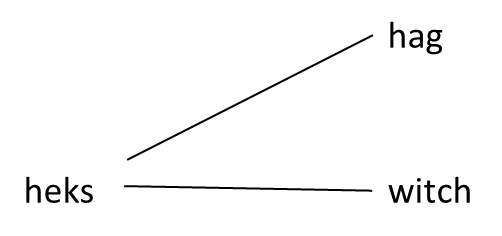
\includegraphics[height=.3\textheight]{figures/Vandevoorde2-img2.png}
\begin{forest} for tree={grow=east}
[heks [witch] [hag] ]
\end{forest}
\caption{\label{fig:key:3}Translational correspondence}
\end{figure}

Subsequently, the lexical sub-senses of \textit{heks} could be expressed as contrastive pairs: $\langle$heks, hag$\rangle$, and $\langle$heks, witch$\rangle$. Within a translational approach, these \textit{pairs} (called \textit{sets} when several languages are involved) can be seen “as a kind of \textit{semantic} \textit{features}, [...] assignable to lexical items, both to the items they were derived from, and to others, which may inherit them [...]” (\citealt[31]{langemets_translations_2005}, my emphasis). Schematically, the “translationally derived features” would then look as in \figref{fig:key:4}.

\begin{figure}[t]
% 
\includegraphics[height=.3\textheight]{figures/Vandevoorde2-img3.png}
\begin{forest} for tree={grow'=east,align=center}
[ heks\\{[}heks|hag{]}\\{[}heks|witch{]} [hag\\{[}hegs|hag{]}] [witch\\{[}heks|witch{]}]  ]
\end{forest}
\caption{\label{fig:key:4}Translationally derived features}
\end{figure}

To sum up, semantic information can be obtained from \textit{translationally} \textit{derived} \textit{features}:

\begin{quote}
Intuitively, the features encode subsenses that the lexical items share with each other. In this way the features become \textit{classificatory} \textit{devices}, grouping lexical items together according to shared semantic properties (\citealt[31]{langemets_translations_2005}, my emphasis).
\end{quote}

\hspace*{-1.49399pt}In a classical structuralist approach, the semanticist would describe word meaning via a \textit{componential analysis}, in which he assigns \textit{semantic features} to words, in order to understand their interrelations \citep[28]{langemets_translations_2005}. While it is true that from a purely structuralist point of view translations could never be used as contrastive semantic informants – because different languages carve up the world or a same semantic field in different ways – Dyvik observes that these differences in carving up the same field are reflected “in the fact that this translational relation is not one-to-one” \citep[29]{langemets_translations_2005} and are semantically informative: contrastive differences can be a reflection of difference(s) (in classification) of semantic properties. Dyvik explicitly states that meaning can be inferred from the \textit{translational relation} between a source language (lexeme\slash structure) and its translation:

\begin{quote}
Corresponding sets of terms in two languages are connected by a relation of translation \citep[29]{langemets_translations_2005}.
\end{quote}

\begin{quote}
The translational relation between the signs of two languages (interrelating ``linguistically predictable translations'') is an instance of the sharing of meaning properties across languages \citep[217]{hasselgard_complexity_1999}.
\end{quote}

In other words: a \textit{translational} \textit{relation} cannot exist between an LPT and its source language lexeme if these two do not share any meaning properties \citep[218]{hasselgard_complexity_1999}. Translational properties can be ``easily'' accessed – at least more easily than the much more abstract meaning properties – by investigating source texts and their translations. We can therefore  try to “define (some) meaning properties in terms of translational properties rather than the other way around (as is common)” \citep[218]{hasselgard_complexity_1999}. In Dyvik’s view – which will adopted for the extension of the SMM (see \sectref{sec:3.4}) – semantic features can be derived from translational data: alternative translations are related to different aspects or related sub-senses of the meaning of a word under scrutiny \citep[31]{langemets_translations_2005}, and can divide up the semantic potentiality of the given word \citep[31]{langemets_translations_2005}. In this way, “sets of translationally corresponding items across languages [can be seen] as \textit{the} \textit{primitives} \textit{of} \textit{semantic} \textit{descriptions}” \citep[31]{langemets_translations_2005}, and the contrastive pairs can be considered as semantic features, assignable to lexical items \citep[31]{langemets_translations_2005}.

\subsubsection{Ivir and Dyvik} 
\label{sec:2.3.4.3}  
Although Dyvik’s mirroring method shows quite some resemblances to Ivir’s ideas about contrastive correspondents and back-translation, Dyvik seems to develop his method independently of Ivir’s previously established notions. Dyvik’s and Ivir’s proposals are similar in that they (i) each use a mechanism which allows them to select only those translational data which they find suitable and ``safe'' for contrastive analysis; and (ii) treat the relation of translational correspondence as a symmetric relation “disregarding the direction of translation” \citep[314]{aijmer_translations_2004}, a viewpoint which is in line with their research goal and seems for both Ivir and Dyvik the methodologically right thing to do: in their contrastive view, pairs of translations are informative tools used for their dynamics to move between languages in a meaning-preserving way, informing the researcher about meaning, while the influence of the task of translation itself is brought down to a minimum, so that the data are as contrastively pure as possible. From a point of view of translation studies though, the translational relation is clearly asymmetric and this has been proven via the same practice of back-translation: “[m]ultiple examples from the practice of back translation have proven that translation pairs are not symmetric and translation through several languages make the lack of transitivity similarly apparent (see e.g. \citealt{Levy1989})” \citep[211]{halverson_concept_1997}. Since the current study focuses on translation itself, and not merely on its exploitation as a (logical) tool, the asymmetry of the translational relation will necessarily have to be taken into account.

One could wonder why such an effort is made here to present Dyvik’s\ia{Dyvik, Helge@Dyvik, Helge} technique, if in fact Ivir’s previously formulated ideas were so similar. There are several important reasons to prefer the SMM to Ivir’s ``pure'' back-translation as a basis for this methodological tool. First, Dyvik makes an important link between a technique, back-translation, and a specific research objective: lexical semantic research, an objective which I share with Dyvik. As a matter of fact, Dyvik operationalizes Ivir’s intuition that each L\textsubscript{2} correspondent will be related to a number of other L\textsubscript{1} items too, besides the L\textsubscript{1} with which the analysis was initiated \citep[478]{dirven_functionalism_1987} by retrieving the “other L\textsubscript{1} items” in an additional corpus-based retrieval step (called the inverse T-image). Second, as \citet[25]{ebeling_patterns_2013} rightly remark, Ivir never explains the procedure of back-translation in detail, which makes it difficult to know whether he applies the method with a parallel corpus, or if back-translation is done on the basis of the analyst’s translational intuitions. For Dyvik on the contrary, the use of (parallel) corpora is an obvious step, explicitly mentioned in his design. Again, I follow Dyvik’s proposal to explicitly put forward a parallel corpus approach for research in lexical semantics of translation. Finally, Dyvik further develops and exploits the notion (which was also mentioned by Ivir, but not exploited) of \textit{overlap} to ensure the semantic relatedness between the yielded lexemes. Overlap is part of the procedure of back-and-forth translation, and forms an additional dimension which will be used in the extended version of the SMM (see \sectref{sec:3.4}).

\subsubsection{The SMM in contrastive linguistic studies}\label{sec:2.3.4.4}\largerpage[2]
Within contrastive, corpus-based studies, Aijmer and Simon-Vandenbergen have drawn extensively on Dyvik’s idea of using translations as “mirrors” in semantic field research. They mainly focused on discourse particles \citep{simon-vandenbergen_english_2013}, pragmatic markers \citep{simon-vandenbergen_expectation_2002,aijmer_model_2004,fischer_pragmatic_2006} and adverbs \citep{simon-vandenbergen_semantic_2007,simon-vandenbergen_english_2013}.\footnote{\citet{mortier_adversative_2009} were inspired by the work of Aijmer and Simon-Vandenbergen and carried out a “mirror-analysis” for adversative discourse markers. They combine different types of corpora (parallel and comparable, with written and spoken data) to arrive at a “semantic profile” for the discourse markers under study. They emphasize that their application of the “mirror analysis” serves to establish “the field of formal equivalents in one language or across languages” \citep[309]{mortier_adversative_2009}. According to the researchers, a mirror analysis “consists of back-and-forth translations of a given item from the source language to the target language, and from the target language back to the source language”. Their application of the procedure in fact answers perfectly to Ivir’s \textit{back-translation} procedure for the retrieval of \textit{formal correspondents} (and this is also the goal of Mortier and Degand), so their method stands much closer to Ivir’s contrastive notion than to Dyvik’s lexical-semantic tool.} In line with the cautiousness which contrastive researchers usually show when employing translational data, Aijmer and Simon-Vandenbergen relied on Dyvik’s argumentation to legitimately incorporate the supplementary information which translations are able to provide about semantic similarity into their analysis. They show an interest in using the back-and-forth translations as a \textit{tertium} \textit{comparationis} (\citealt[16]{simon-vandenbergen_expectation_2002}, \citealt[1795]{aijmer_model_2004}), but their main interest in Dyvik’s proposal stems from its aptitude to construct and compare semantic fields (\citealt[1131]{aijmer_discourse_2003}; \citeyear[1782]{aijmer_model_2004}; \citealt[13]{simon-vandenbergen_expectation_2002}). A number of adaptations and specifications are made by Aijmer and Simon-Vandenbergen to Dyvik’s original method. Firstly, Aijmer and Simon-Vandenbergen always use at least three languages; i.e. the language under study (English) and two mirror languages: either Dutch and Swedish \citep{aijmer_model_2004}, or Dutch and French \citep{simon-vandenbergen_english_2013} or even four mirror languages (Dutch, Swedish, French and German) at once \citep{simon-vandenbergen_semantic_2007}, whereas Dyvik uses two languages: one language under scrutiny and one pivot language. Aijmer and Simon-Vandenbergen in fact combine the resulting translations from two mirror analyses (a mirror exercise can only be carried out with one language at a time) into one resultant relational field. If, for instance, Dutch and Swedish are used as pivot languages, this double mirror allows them to compare the “overlapping translations back into English”. “Overlapping translations” are interpreted here as those translations back into English which are obtained as translations of both Swedish and Dutch source lexeme(s). The result is a set of English lexemes, overlapping\footnote{Note that this interpretation of overlap differs from the interpretation of the notion in this study.} between Dutch and Swedish. In this way, Aijmer and Simon-Vandenbergen compare  the number of identical translations (from Dutch or Swedish) into English yielded in what they call “the second translation image” \citep[1796]{aijmer_model_2004}, which corresponds to Dyvik’s step of the inverse T-image (see \sectref{sec:2.3.4.3}). Combining different mirror images into one result also implies that data are obtained from different corpora and need to be combined while staying comparable.

Secondly, whereas Dyvik’s “ranking of signs in a semantic field” is done “quite independently of frequency of occurrence”,\footnote{“(except that a lexeme of course has to occur at least 32 times in the corpus in order to be a member of 32 subsets)” \citep[73]{johansson_translational_1998}.} and based on the “overlap relations among \textit{t}{}-images” \citep[73]{johansson_translational_1998}\footnote{Recall the quote at the beginning of this section, stating that overlapping first \textit{t}{}-images do not guarantee that two lexemes indeed pertain to the same field “since the shared L2 sign may be ambiguous between an ‘\textit{a}{}-sense’ and a ‘\textit{b-}sense’ with no close relationship between them” \citep[72]{johansson_translational_1998}. In order to ensure that two lexemes do pertain to the same field, Dyvik proposed the technique of back-and-forth translation up to the level of the \textit{second} \textit{T-image} (the necessity of the \textit{second} \textit{T-image} will be further explicated in the methodological chapter of this study).} \citet{aijmer_model_2004} use frequency information to differentiate the items of a lexical set (obtained via a mirror analysis as translations of one particular marker in one language under scrutiny): 

\begin{quote}
Such paradigms or lexical sets show, for example, which translations are more frequent or prototypical, and which are less frequent or even ``singleton'' translations \citep[1785--1786]{aijmer_model_2004}.
\end{quote}

The (relative) frequency information of correspondences is used to distinguish between prototypical equivalents and more context-bound correspondences \citep[8]{simon-vandenbergen_semantic_2007}, but frequency information is not as such integrated in the visualized results which represent the translation networks \citep[250--253]{simon-vandenbergen_semantic_2007}. The researchers choose to only consider salient correspondences in their translation network “in principle the five most frequent ones, though individual decisions had to be taken in view of the large differences in absolute and relative frequencies in separate tables” \citep[248]{simon-vandenbergen_semantic_2007}. This problem is a direct consequence of the fact that different corpora had to be combined for this application. Thus, Aijmer and Simon-Vandenbergen do not neglect frequency information, but the resultant contrastive translation networks are not (directly) based on the frequencies of the correspondences; the lines which link up the contrastive lexemes in the translation networks in fact only reflect cross-linguistic translation overlap,\footnote{This modus operandi is further confirmed in \citet[93--94]{simon-vandenbergen_english_2013}, where the relation (within a ``mirror analysis'') between French or Dutch equivalents and English lexemes is indicated by one cross if such a relation exists and two crosses if the relation was recorded more than once.} which is a different kind of overlap from Dyvik’s notion. A distinction is made between full lines to mark the prototypical correspondences, and broken lines which show “correspondences which are not prototypical but [...] still recurrent enough to be included” \citep[248]{simon-vandenbergen_semantic_2007}.\largerpage[2]

To sum up, Aijmer and Simon-Vandenbergen propose a “translation-based variant of semantics based on data from translation corpora” \citep[7]{simon-vandenbergen_semantic_2007} for which they draw on Dyvik’s semantic mirrors method. Interesting adjustments to the technique consist in their use of multiple languages to arrive at a final semantic map as well as the integration of frequency information, although without statistically incorporating this information into the analysis.

\subsubsection{The SMM in other domains of linguistics}\largerpage\label{sec:2.3.4.5}  
The SMM has also drawn the attention of researchers in Natural Language Processing. \citet{ganter_conceptual_2005} have proposed to model the SMM with Formal Concept Analysis, using concept lattices to visualize semantic relatedness instead of the Venn diagrams proposed by Dyvik. \citet{elden_computing_2013} propose to visualize the semantic relations which come from semantic mirrors via Spectral Graph Partitioning. In addition to this, the SMM has been compared, within the realm of computational linguistics, with its ``competing'' distributional techniques for automated thesaurus construction. \citeauthor{butz_comparing_2011} concluded that “with respect to synonyms, [...] mirror translations provide a better filter than syntactic distribution similarity” (\citeyear[333]{butz_comparing_2011}). It is beyond the scope of this study to further comment on these computational applications, but the fact that the SMM has been applied both in more theoretical contrastive linguistic works on the one hand and in computational applications on the other at least shows that the ideas underlying the SMM have found support in both theory and practice.

\subsection{Conclusion}
\label{sec:2.3.5}  
Back-translation is a technique that can be used as a contrastive linguistic tool. It enables the researcher to isolate formal correspondents (renamed and re-defined by Ivir as contrastive correspondents) and to detect semantic relationships between lexemes in one language. An application of back-translation via semantic mirroring offers – in theory – the possibility to investigate semantic relationships in translated and non-translated language. Although the SMM has indeed the potential to lay bare meaning relationships, a number of issues remain unsolved. First, a operationalizable notion of translation equivalence allowing for valid comparisons between translated to non-translated language is still to be defined. Both Dyvik and Ivir established equivalence on the basis of a symmetric notion of the translation relation, but the idea that equivalence is symmetric is incompatible with the viewpoint of CBTS which is taken in this book. Second, the SMM was originally a method for thesaurus building and is therefore not ``equipped'' to carry out comparisons of the semantic relationships it lays bare amongst different language varieties. Thirdly, provided that the first two issues can be overcome, a theoretical framework within which those comparisons can be interpreted, is still missing. Solutions to each of these problems can be found within corpus-based semantics.

\section{Corpus semantics}
\label{sec:2.4}  
Various theoretical insights from different areas of corpus-based semantics are brought together in this section. These insights are needed to underpin the methodology which will be presented in \chapref{sec:3}. Three elements are still missing: (i) an acceptable notion of translation equivalence (applicable within the SMM and allowing an asymmetric translational relation), (ii) an insightful means to compare semantic relationships in translated and non-translated language and (iii) a theoretical framework within which such comparisons can be interpreted. Corpus(-based) semantics is an extremely vast area of research. I will therefore only touch upon those domains that are immediately relevant to theoretically underpin the three aspects cited above.

In the first part of this section (\sectref{sec:2.4.1}), I deal with the notion of translational equivalence as it was developed in Word Sense Disambiguation. By considering translational equivalence according to its WSD-based definition, the notion can also be used when the translational relation is not considered symmetric (as is the case in this study).

In \sectref{sec:2.4.2}, I will show that the semantic relationships revealed on the basis of the translational equivalence hypothesis can be understood in terms of distances and captured in so-called Semantic Vector Spaces. Statistical visualization methods can consequently be used as “an intuitive interface” \citep*[17]{heylen_looking_2012} to study semantic relationships in fields of translated and non-translated language.

In \sectref{sec:2.4.3}, I will explore how the idea of a “prototype model of category structure” – considered as one of the important contributions of cognitive semantics to the study of word meaning \citep[577]{allan_lexical_2013} – can form the theoretical background against which the semantic relationships within the semantic field under study can be interpreted.

\subsection{Translational equivalence in Word Sense Disambiguation}
\label{sec:2.4.1}  
The idea that a procedure such as back-translation based on translation equivalence introduced in \sectref{sec:2.3} can be used to lay bare semantic relationships also exists within corpus-based semantics. The derivation of semantic relationships on the basis of translational equivalence is put into practice within Word Sense Disambiguation – a name commonly given in the field of computational linguistics to the task of “computationally determining which ``sense'' of a word is activated by the use of the word in a particular context” \citep[1]{agirre_word_2007}.

In WSD, unsupervised corpus-based methods\footnote{The different approaches to WSD are classified according to their main source of information: knowledge-based methods use sources such as dictionaries and thesauri, unsupervised methods collect information from raw unannotated corpora and include methods using word-aligned corpora which extract cross-linguistic information; (semi-)supervised methods train from annotated corpora, or use them to seed in a bootstrapping process \citep[12]{agirre_word_2007}.} are either based on the distributional hypothesis, or, alternatively, on the idea of translational equivalence \citep{agirre_word_2007}. So-called distributionalist methods are often summarized in John R. Firth’s well known words “You shall know a word by the company it keeps” \citep[11]{firth_synopsis_1957}.\footnote{In computational linguistics, the distributional hypothesis is also commonly attributed to \citet{anscombe_philosophical_1953}, \citet{harris_distributional_1954}  or \citet{weaver_translation_1955} \citep[142--143]{turney_frequency_2010}.} The translation equivalence hypothesis is based on the idea that a word can be known by the translational company it keeps. Translational equivalence methods were introduced into computational linguistics because of their relevance for machine translation \citep[134]{agirre_unsupervised_2007}, one of the earliest fields of application of WSD. The reliability of translational equivalence has received direct evidence from WSD: according to \citet[1]{ide_automatic_2001} “sense distinctions derived from cross-lingual information correspond to those made by human annotators, especially at the coarse grained level” and “the reliability of sense assignments at finer-grained levels is comparable for human annotators and those produced automatically with cross-lingual data”.

While in lexical semantics, distributional approaches are widely applied,\footnote{In lexical semantics and lexical variation studies (e.g. \citealt{peirsman_automatic_2010}), the distributionalist idea has led to the advent of (semi-)automatic retrieval methods of semantically similar words such as latent semantic analysis \citep{landauer_solution_1997}, first and second-order bag-of-words models (\citealt{manning_foundations_1999}) and the behavioral profiles method (\citealt{divjak_ways_2006, evans_behavioral_2009}).} methods that rely on translational equivalence as a meaning-structuring device have not yet had much uptake. Admittedly, the distributional hypothesis has opened the way to a myriad of methodological possibilities and fine-grained analytical tools (which do not seem to have reached their limitations yet) so the ``need'' to rely on an alternative hypothesis can seem somewhat obsolete. However, if one is interested in investigating the semantics of translated language (in comparison to non-translated language), the translational hypothesis might be an appropriate starting point. In fact, the idea of translational equivalence can be rather straightforwardly related to the widely used distributional approach. We could easily reformulate the acceptability of translational equivalence in distributionalist terms, i.e. with respect to the (additional or alternative) contextual disambiguation possibilities that translations offer: the addition of information from a second language (a translation) about a lexeme under scrutiny (the source language lexeme) – which stands in a translational relation to that lexeme – can be seen as ``addition of context''. Translational equivalence methods could therefore be said to form – at least conceptually, and at least for research focusing on lexical semantic investigations in translation studies – a possible alternative for or addition to the existing distributional methods, as is already the case within WSD.

Now that we have argued in favor of the conceptual acceptability of translational equivalence for lexical semantic research in translation, we need to understand exactly how translational equivalence works within WSD. WSD methods based on translational equivalence unsurprisingly use translations as information source for disambiguation:

\begin{quote}
methods based on translational equivalence rely on the fact that the different senses of a word in a source language may translate to completely different words in a target languages \citep[134]{agirre_unsupervised_2007}.
\end{quote}

In machine translation (the field where WSD researchers initially got the idea for translational equivalence), “the ambiguity of a source word is [...] given by the number of target representations for that word in the bilingual lexicon of the translation system” \citep[132]{dagan_two_1991}. For example, if in a machine translation task, the correct sense of the English lexeme \textit{bank} needs to be selected, the conditio sine qua non to perform this task (correctly) is that the system disposes of the necessary information to differentiate between the different senses of \textit{bank.} The distinctive senses of \textit{bank} can be assigned to the lexeme “by producing all the [French] alternatives for the lexical relations involving [bank]” \citep[131]{dagan_two_1991}. The French translation \textit{banque} distinguishes the `financial institution' sense of \textit{bank}, whereas the French \textit{rive} reveals the `riverside' sense of \textit{bank.} Schematically, the sense assignment looks as in \figref{fig:key:5}.

Given that the lexeme \textit{bank} now possesses two possible senses, it has become possible to select the sense “which corresponds to the most plausible [French] lexical relations” \citep[131]{dagan_two_1991} and consequently to select the contextually correct target word.

Not all ambiguities can be resolved through ``simple'' translational equivalence. For instance, at least two senses of the Dutch lexeme \textit{school} cannot be disambiguated while using English translations: the `educational institution' sense of Dutch \textit{school} translates in English as \textit{school}, and the `group of fishes' sense of Dutch \textit{school} also translates into English as \textit{school}, hence, ambiguity remains unresolved (\figref{fig:key:6}). In these cases, it is proposed to add a third language \citep[132]{dagan_two_1991}. In this particular case, adding French would help, as the `group of fishes' sense translates in French as \textit{banc}, and would reveal this additional sense (\figref{fig:key:7}).

\begin{figure}
% 
\includegraphics[height=.3\textheight]{figures/Vandevoorde2-img4.png}
\begin{forest}for tree={grow=east,align=center}
    [bank  [\textit{rive}\\{[}riverside{]}] [~~~~~~~~~~~~~~~~~~~~,name=dummy,no edge [bank\\{[}\textit{banque}{],} {[}\textit{rive}{]},base=center,edge=->]] [\textit{banque}\\{[}financial institution{]}] ]
\end{forest}
\caption{\label{fig:key:5}Different senses of the English lexeme \textit{bank} are assigned based on its French translations}
\end{figure}

\begin{figure}
% 
\includegraphics[height=.3\textheight]{figures/Vandevoorde2-img5.png}
\begin{forest} for tree={grow=east,align=center}
[school\textsubscript{Du} [\textit{school}\textsubscript{Eng}\\{[}group of fishes{]}] [~~~~~~~~~~~~~~~~~~~~,name=dummy,no edge [school\textsubscript{Du}\\{[}\textit{school}{],} {[}\textit{school}{]},base=center,edge=->]]  [\textit{school}\textsubscript{Eng}\\ {[}educational institution{]}] ]
\end{forest}
\caption{\label{fig:key:6}Unresolved disambiguation via one language}
\end{figure}

\begin{figure}
% 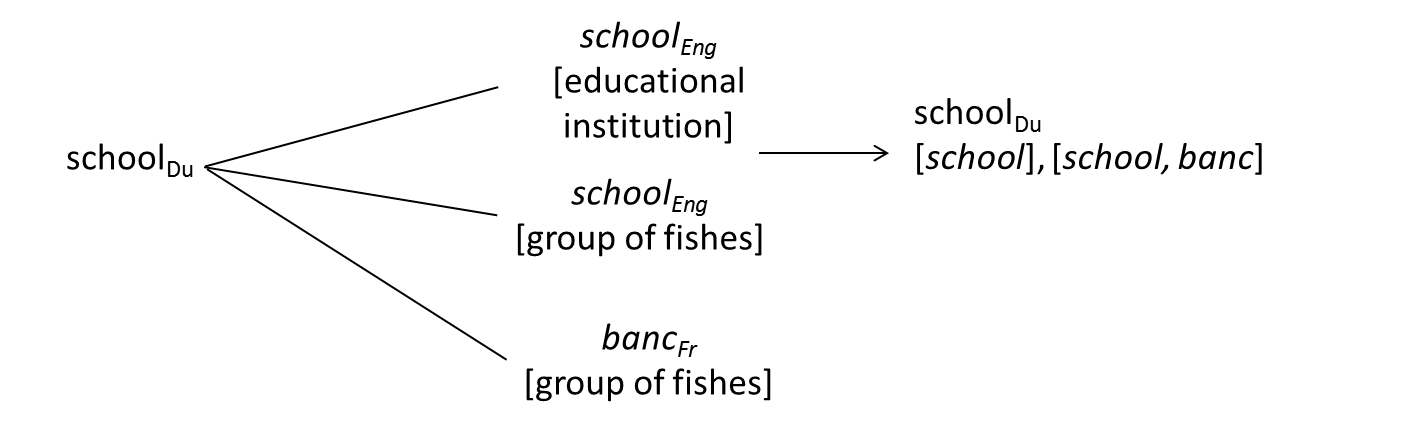
\includegraphics[height=.3\textheight]{figures/Vandevoorde2-img6.png}
\begin{forest} for tree={grow=east,align=center}
[school\textsubscript{Du}\\\vphantom{jh}~ [\textit{banc}\textsubscript{Fr}\\{[}group of fishes{]}] [\textit{school}\textsubscript{Eng}\\{[}group of fishes{]},base=center [school\textsubscript{Du}\\{[}\textit{school}{],} {[}\textit{school, banc}{]},base=center,edge=->]]  [\textit{school}\textsubscript{Eng}\\ {[}educational institution{]}] ]
\end{forest}
\caption{\label{fig:key:7}Resolved disambiguation via two languages}
\end{figure}

While adding a language or even several languages \citep{gelbukh_five_2013}, has proven to be an effective way to enhance the WSD procedure, it is also conceptually possible to rely on a single language and still arrive at the disambiguation of the different senses. This can be done by applying the procedure of back-and-forth translation following the SMM. Within the SMM, the translational relation is, however, considered as symmetric, an idea which is incompatible with my point of view that translation is necessarily asymmetric (see \sectref{sec:3.4.1}). The idea of a symmetric translation equivalence relation is, however, not a prerequisite to carry out back-and-forth translation with the SMM. In fact, disambiguation via the SMM can rely on the same basic idea as disambiguation via several languages in WSD, which states that the different senses of a word are determined by considering only those distinctions that are lexicalized cross-linguistically \citep[54]{agirre_making_2007}. By considering the relation of translational equivalence in the SMM as identical to the one in a WSD disambiguation task with several languages, i.e. not necessarily symmetric and lexicalized cross-linguistically – the SMM can be used for the disambiguation task carried out in this study.

\subsection{Vector Space Models}
\label{sec:2.4.2}  
The SMM can be used to reveal semantic relationships, but it cannot be “readily” used to compare the obtained relationships amongst different language varieties. The same holds for WSD: it is a (computational) task to determine sense distinctions, but it does not offer solutions as to how the disambiguated senses can be objectively compared to each other. Objective comparisons would indeed require objective visualization methods, which neither the SMM nor WSD straightforwardly offer. In this section, I will turn to linguistic semantics and corpus-based cognitive semantics, which are mainly occupied with the empirical study of lexical meaning. Semantic relationships revealed on the basis of the translational equivalence hypothesis can be understood in terms of distances and captured in so-called Semantic Vector Spaces (SVS). Statistical visualization methods can consequently be used as “an intuitive interface” \citep[17]{heylen_looking_2012} to explore the semantic relationships in fields of translated and non-translated language “captured by an SVS” \citep{heylen_looking_2012}.

In linguistic semantics and corpus-based cognitive semantics, the perceived difficulties to introspectively analyze meaning and meaning differences have led to the development of “a methodology for empirical research in cognitive linguistics that is based on thorough quantitative analysis of corpus data” \citep[91]{kristiansen_methodological_2008}. Data are derived from or gathered via corpora and quantitatively analyzed using methods that are “methodologically similar” to work in computational linguistics or information retrieval \citep[6]{gries_introduction_2006}. \citet[242]{riemer_sense_2016} and \citet{glynn_empirical_2010} discern three major perspectives: experimental research, the referential method and the distributional, corpus-based approach. My own proposition to reveal semantic relationships on the basis of the translational hypothesis can be fitted in with the distributional, corpus-based approaches to the empirical study of lexical meaning as translations can be considered as an alternative for an additional type of context.

According to \citet[242--243]{riemer_sense_2016}, the distributionalist corpus-based\linebreak method takes three main forms: one in the tradition of Sinclair, a second one following the behavioral profile approach and a third form, called the semantic vector space approach. In Sinclair’s tradition, statistical methods are used to “identify semantically relevant contextual clues in the corpus” \citep[242]{riemer_sense_2016} after which the “semantic characterization” of the words and expressions is usually analyzed manually \citep[242]{riemer_sense_2016}. The behavioral profile approach takes the opposite direction: potentially interesting features are first tagged manually or semi-automatically, after which statistical techniques are applied to “classify the occurrences into distinctive senses and usages” \citep[243]{riemer_sense_2016}. Various statistical techniques have been used within this approach, e.g. hierarchical cluster analysis by \citet{gries_corpus-based_2006} and \citet{divjak_structuring_2010} and correspondence analysis by \citet{glynn_empirical_2010} \citep[243]{riemer_sense_2016}. The third approach discerned by Geeraerts, the semantic vector space approach, uses quantitative techniques on both levels: contextual clues are first identified in a statistical way; the subsequent “clustering of occurrences on the basis of those clues” is equally carried out statistically \citep[243]{riemer_sense_2016}.

Vector Space Models (henceforth: VSMs) – which are put forward within this semantic vector space approaches – were initially proposed as a solution to the problem of document retrieval in Information Retrieval \citep[495]{lappin_vector_2015}. They can be combined with the distributional hypothesis “as an approach to representing some aspects of natural language semantics” \citep[141]{turney_frequency_2010}. \citet[212]{szmrecsanyi_semantic_2014} explain how VSMs can be combined with the distributional hypothesis:

\begin{quote}
[I]n Vector Space Models, objects are described by \textit{n} quantifiable characteristics. These characteristics make up an $n$-dimensional space in which the objects can be positioned. Every characteristic is thus a dimension. The position of the objects along these dimensions depends on the value that the characteristics have. In a way, these values can be seen as coordinates of a point in the \textit{n}{}-dimensional space, made up by the characteristics. The values of a single point are stored in a so-called vector. Every vector represents the object that is described by its characteristics. The spatial idea that underlies Vector Space Models does not restrict the objects to tangible items. Indeed, in Distributional Semantics, word meanings are objects, and the characteristics are contexts in which these words appear \citep[212]{szmrecsanyi_semantic_2014}.
\end{quote}

When VSMs are combined with the distributional hypothesis, the quantifiable characteristics of the object (i.e. of the word meaning) are the contexts of the word under scrutiny. Parallel to this proposition, VSMs can now also be combined with the translational equivalence hypothesis: the quantifiable characteristics which make up an $n$-dimensional space are then the translations or the source language lexemes of a word under scrutiny provided that a relationship of translational equivalence has been established (which will be done via the SMM++) between the translation\slash source language word and the word under study.

The attraction of the VSMs for semantic research resides in the fact that they can be used to quantify semantic similarity “by applying the spatial idea that underlies the Semantic Vector Space Models” \citep[213]{szmrecsanyi_semantic_2014}. This works as follows:

\begin{quote}
If two objects are very close to each other in an \textit{n}{}-dimensional Semantic Vector Space, then they are bound to have very similar values on a number of dimensions. If two objects behave alike for a large number of characteristics, represented by the dimensions, they must be very similar to each other, with respect to these dimensions. Given that we assume that the dimensions in Semantic Vector Spaces represent the Distributional Semantics of a lemma, spatial closeness of two words translates into semantic similarity between these words” \citep[213]{szmrecsanyi_semantic_2014}.
\end{quote}

Again, the idea that Semantic Vector Spaces can be combined with the distributional hypothesis can be transposed to the translational hypothesis: in order to know how semantically similar two words are in translated and non-translated language, the spatial proximity between those two words can be measured in both varieties. For instance, the semantic similarity between \textit{stoel} `chair' and \textit{bank} `bench' can be measured in translated Dutch and compared to the semantic similarity between those same two lexemes in non-translated Dutch. In translated Dutch, \textit{stoel} `chair' and \textit{bank} `bench' are translations and each lexeme is represented by a vector containing all possible source language words obtained from a corpus (as frequency values). For non-translated Dutch, \textit{stoel} `chair' and \textit{bank} `bench' are source language lexemes and each lexeme is represented by a vector containing all possible translations obtained from a corpus (as frequency values). Following the idea that “spatial closeness of two words translates into semantic similarity between these words” \citep[213]{szmrecsanyi_semantic_2014}, we can compare the distances between \textit{stoel} `chair' and \textit{bank} `bench' in both varieties and consequently compare the semantic similarity between the two lexemes for both translated and non-translated Dutch. 

In a large, corpus-based study such as this one, each translation or source language lexeme will be represented as a row in a frequency table and each characteristic of the $n$-dimensional space (source language lexeme or translation) will be represented as a column variable in a data matrix. If one wants to see “what kind of semantics” \citep[17]{heylen_looking_2012} is hidden within such potentially huge data matrices “an intuitive interface to explore the semantic structure captured by an SVS” \citep[17]{heylen_looking_2012} will be needed. Such an interface (a visualization) can then be obtained via statistical analysis of those data matrices. In this study, Correspondence Analysis and Hierarchical Cluster Analysis will be applied to yield such visualizations (see \sectref{sec:3.6}).

\subsection{Corpus-based cognitive semantics}
\label{sec:2.4.3}  
In linguistic semantics, thorough quantitative corpus analyses have been combined with theoretical concepts of cognitive linguistics, mostly in an attempt to arrive at a more empirical account of lexical meaning. \citeauthor{kristiansen_methodological_2008} compared the work developed by two groups of researchers who have “relatively independently [developed] the methodology of “cognitive linguistically inspired” quantitative corpus analysis” \citep[92]{kristiansen_methodological_2008}.\footnote{The comparison between the two approaches will not further be discussed here, but see \citet{kristiansen_methodological_2008}. Briefly, the differences between the approaches situate themselves on the level of the phenomena under investigation, explanatory approaches and the exact statistical technique employed \citep[92--93]{kristiansen_methodological_2008}.} \citet{gries_corpus-based_2006} explains that, by bridging the gap between cognitive studies and corpus-based studies, rather than focusing on the distributional characteristics of different word senses, it should become possible to be informed about “how different word senses are related” \citep[57]{gries_corpus-based_2006}. The integration of a cognitive linguistic framework within a corpus linguistic study is moreover believed to lead to more “theoretical sophistication” \citep[16]{gilquin_corpus_2010}. In this section, a “prototype model of category structure” will be proposed as the theoretical basis for the interpretations of the obtained visualizations (see \chapref{sec:4}). The “prototype model of category structure” is considered as one of the important contributions that cognitive semantics has made to the study of word meaning \citep[577]{allan_lexical_2013}. In the first part of this section (\sectref{sec:2.4.3.1}), I will zoom in on the notion of prototypicality so that it can be used in an unproblematic way to further describe and interpret the results presented in the subsequent chapters of this study. In the second part (\sectref{sec:2.4.3.2}), I will show how Divjak’s proposal to opt for a prototype-based categorization for low-contrastive verbs expressing abstract concepts also seems to be the better choice for this study. In addition, I will comment on Divjak’s two proposals of internal category organization (schematic or radial structure). Just like Divjak, I will also prefer a radial category organization.

\subsubsection{A prototype-based view and prototype effects}
\label{sec:2.4.3.1}  
The development of prototype theory received its most important impetus from psycholinguistic research conducted by Eleanor Rosch and colleagues in the 70s \citep{rosch_cognitive_1975,Rosch1978,margolis_principles_1999,rosch_family_1975}. One of Rosch’s most important findings was that “[m]ost, if not all, categories do not have clear cut boundaries” \citep[196]{margolis_principles_1999}. The idea of fuzzy category boundaries seemed, however, not easy to connect to the ``dictate'' of cognitive economy that saw categories as “being as separate from each other and as clear-cut as possible” \citep[196]{margolis_principles_1999}. Rather than intending to achieve cognitive economy via “formal, necessary and sufficient criteria for category membership”, one could, alternatively, opt to marry fuzzy boundaries with cognitive economy by “conceiving of each category in terms of its clear cases rather than its boundaries” \citep[196]{margolis_principles_1999}. Prototypes of categories are then “the clearest cases of pry membership defined operationally by people’s judgments of goodness of membership in the category” \citep{margolis_principles_1999}. Rosch thus considered perception of typicality difference and hence also degree of prototypicality as an empirically verified fact. Given this empirical fact, Rosch went on to ask precisely “what principles determine which items will be judged the more prototypical?” \citep[197]{margolis_principles_1999}. Her hypothesis was that “prototypes develop through the same principles such as maximization of cue validity and maximization of category resemblance as those principles governing the formation of categories themselves” \citep{margolis_principles_1999}. Support for this hypothesis can be found in \citet{rosch_family_1975}, who showed that “the more prototypical of a category a member is rated, the more attributes it has in common with other members of the category and the fewer attributes in common with members of the contrasting categories” \citep[197]{margolis_principles_1999}.

Outside the field of psycholinguistic research, Rosch’s findings have further evolved and influenced psycholexicology on the one hand, and from the mid-1980s onwards also (general) linguistics \citep[578]{allan_lexical_2013}. As far as cognitive linguistics is concerned, prototype theory is even seen as “one of its cornerstones” \citep[145]{Geeraerts2006}. According to Geeraerts, within linguistics, Rosch’s conclusions that “perceptually based categories do not have sharply delimited borderlines” developed into “a more general prototypical view of natural language categories, more particularly, categories naming natural objects” \citep[578]{allan_lexical_2013}. Geeraerts further summarizes the application of prototype theory to the domain of linguistics as follows:

\begin{quote}
The theory implies that the range of application of such categories is concentrated round focal points represented by prototypical members of the category. The attributes of these focal members are the structurally most salient properties of the concept in question; conversely, a particular member of the category occupies a focal position because it exhibits the most salient features \citep[578]{allan_lexical_2013}.
\end{quote}

According to Gilquin, the importance of the introduction of the notion of prototypicality in linguistic theory lies in the fact that categories do not ``need'' to be described any longer by lists for necessary and sufficient properties, but can instead be described according to more central and more marginal category members \citep[160--161]{gilquin_place_2006}. Prototypicality was furthermore extended beyond concrete objects to more abstract categories such as past tense and syntactic constructions (\citealt{gilquin_place_2006}, referring to \citealt{taylor_linguistic_1989}).

The use of the notion within linguistic theory is, however, not uncontroversial. Geeraerts shows that prototypicality is itself “a prototypical notion with fuzzy boundaries” \citep{Geeraerts2006}. Prototypicality, according to Gilquin, needs to be considered as follows:

\begin{quote}
a multi-faceted concept, bringing together (1) theoretical constructs from cognitive literature and relying on deeply-rooted neurological principles such as the primacy of the concrete over the abstract, (2) frequently occurring patterns of (authentic) linguistic usage, as evidenced in corpus-data, (3) first-come-to mind manifestations of abstract thought, as revealed through elicitation tests and (4) possibly other aspects that contribute to the cognitive salience of a prototype \citep[180]{gilquin_place_2006}.
\end{quote}

By defining prototypicality along these different lines, Gilquin tries to incorporate the four hypotheses uttered by \citet{geeraerts_where_2006} as possible answers to the question: “where does prototypicality come from?”. These four hypotheses run as follows: First, the physiological hypothesis: prototypicality is considered as the result of the physiological structure of the perceptual apparatus \citep{moore_internal_1973}. The problem with this hypothesis is that it is difficult to apply to concepts without physiological basis \citet[28]{geeraerts_where_2006}. Second, the referential hypothesis: prototypicality as the result of the fact that “some instances of a category share more attributes with other instances of the category than certain peripheral members of the category” \citet[28]{geeraerts_where_2006}. This hypothesis is also referred to as the “family resemblance model of prototypicality” \citep{rosch_family_1975}. The number of shared attributes among the objects, events, ... a concept can refer to, can allow the researcher to compute differences in salience \citep[29]{geeraerts_where_2006}. Thirdly, according to the statistical hypothesis, the prototype is that member of a category which is most frequently experienced. \citet[29]{geeraerts_where_2006} adds that the second and the third hypothesis can be combined: one can ascribe weights to category attributes on the combined basis of family resemblance and relative frequency \citep{rosch_cognitive_1975}. Finally, the fourth hypothesis is the psychological (also called functional) hypothesis which states that “it is cognitively advantageous to maximize the conceptual richness of each category through the incorporation of closely related nuances into a single concept because this makes the conceptual system more economic” \citep[28]{geeraerts_where_2006}.

I follow Gilquin’s “multi-faceted” view on prototypicality, which incorporates Geeraerts' four hypotheses. However, the following question arises: if a pro\-to\-type-based view on language is taken and claims are made about the semantic relationships within the presumably prototype-based semantic fields, how can one be sure that the chosen method will actually render a prototype-based structure? Given the corpus-oriented scope of this work, the most straightforward way of ``ensuring'' that the yielded semantic fields will be prototype-based is to integrate both Geeraerts’ second (family resemblance\slash salience) and the third (statistics) hypothesis. In this way, a cognitivist view on prototypicality – “cognitivists tend to consider the prototype as the cognitively most salient exemplar” \citep[159]{gilquin_place_2006} – is united with a corpus-linguistic view which usually considers the prototype as the most frequently corpus-attested item \citep{gilquin_place_2006}. As Gilquin points out, most of the time, both cognitivists and corpus-linguists assume that salience and frequency coincide with one another \citep{gilquin_place_2006}. Although Gilquin does not negate the role of frequency in prototypicality, she also cites \citet[36]{sinclair_corpus_1991} who argues that “for common words, as a rule, the most frequent meaning is not the one that first comes to mind”. In this study, I will not only take frequency as a measure of prototypicality, I will also propose a way to operationalize salience, and I will do so by taking into account the number of overlapping translations. By doing so, I also tackle the problem that “[t]he lack of convergence between salience and text frequency challenges the ability of corpora to serve as a shortcut to cognition” \citep[9]{arppe_cognitive_2010}. By considering translations as attributes, I am able to apply Geeraerts' idea (\citeyear[29]{geeraerts_where_2006}) that the number of shared attributes (overlapping translations) can be used to compute salience. The principle of overlap will be further developed in \sectref{sec:3.4.3.5}. In short, I combine the use of frequency – the statistical hypothesis – and overlap – my operationalization of salience – to determine the status (more prototypical or more peripheral) of the member(s) of the semantic field I plan to visualize.

Geeraerts’ four hypotheses can be linked to a number of prototype effects. Just like Rosch was interested in the principles governing prototypicality judgment, researchers in linguistics too felt the need to differentiate between different phenomena that were all linked in some way to prototypicality (or to one of the previously cited hypotheses about the origins of prototypicality) and consequently prefer to talk about prototype effects rather than about prototype theory \citep[578]{allan_lexical_2013}. Geeraerts sums up a list of four characteristics about which there exists a consensus in the literature on the fact that “these characteristics are prototypicality effects [...] may be exhibited in various combinations by individual lexical items, and [...] may have very different sources” \citep[578]{allan_lexical_2013}. The list of prototypicality effects is determined as follows by Geeraerts:

\begin{quote}
First, prototypical categories exhibit degrees of typicality: not every member is equally representative for a category. Second, prototypical categories exhibit a family resemblance structure, or more generally, their semantic structure takes the form of a radial set of clustered and overlapping readings. Third, prototypical categories are blurred at the edges. Fourth, prototypical categories cannot be defined by means of a single set of criterial (necessary and sufficient) attributes \citep[187]{geeraerts_theories_2010}.
\end{quote}

The existence of these prototypicality effects will need to be taken into account in the development of the methodology (see \chapref{sec:3}). Under the assumption that not every member is equally representative for a category, the method will need to be able to inform about member representativity (this will be done by calculating the distance from each lexeme to its cluster’s centroid, see \sectref{sec:3.6.3}). As far as the family resemblance structure is concerned, it will be integrated by means of the so-called overlap principle. The fuzziness of category boundaries will be dealt with by imposing a minimum threshold for the overlap criterion (see \sectref{sec:3.4.3}) and the remaining fuzziness will be evaluated by assessing the distance of each lexeme to its cluster’s centroid as well as to the centroids of other clusters (see \sectref{sec:3.6.3}). Lastly, the lexeme selection technique based on the SMM takes translations as its attributes – so categories do not need to be defined according to their necessary and sufficient attributes.

\subsubsection{A prototype-based categorization of verbs}
\label{sec:2.4.3.2} 
Divjak remarks that many of the experiments about prototype categorization have been conducted on nouns, so that “[e]xtending prototype categorization to verbs [...] presupposes that knowledge about structures pertaining to nouns might be operative in verbs” \citep[150]{divjak_structuring_2010}. Given a number of differences between nouns and verbs – verbs are not stable\slash time independent, verbs name intangible events, verbs render relational concepts \citep{divjak_structuring_2010} – it is indeed plausible that “conceptual categories associated with verbs and adjectives function differently from those associated with nouns” \citep{divjak_structuring_2010}. According to Divjak, verbs are in general more abstract concepts than nouns and therefore less tangible, making it more difficult to capture them in prototype representations. As far as the intangibility of the verb concepts is concerned, \citet[152]{divjak_structuring_2010} refers to \citet[114]{pulman_word_1983}, who states that verbs will require “more complex and more abstract attributes” than more tangible concepts expressed by nouns (where the prototypical members are those which share most attributes with some members of a category and only some attributes with other, peripheral members). Despite these differences, Divjak indicates that there is “some psychological evidence that people categorize event-related and object-related information in a similar way” \citep[151]{divjak_structuring_2010}. There seems to be no doubt, however, that “categories for intangible relational concepts also display prototype effects” \citep[153]{divjak_structuring_2010}, as is shown by \citet{schmid_cottage_1993,taylor_linguistic_1995,taylor_linguistic_2003,geeraerts_preponderantieverschillen_1985, rudzka-ostyn_where_1988, geeraerts_homonymy_1990} (all cited by \citealt[153]{divjak_structuring_2010}). Divjak concludes that choosing categorization by prototype is “quite adequate for modeling low-contrastive verbs, expressing abstract concepts such as intention, attempt or result [...]” \citep[150]{divjak_structuring_2010}.

Since the semantic domain covered in this study also expresses a rather abstract concept (inchoativity), I believe that the above line of reasoning in favor of prototype-based categorization also holds for this study. Divjak herself uses ID tags to set up behavioral profiles for each of the verbs in her study for prototype identification \citep[158]{divjak_structuring_2010}. My own proposition to operationalize translations as attributes might offer an alternative solution to the ``problem'' of the complexity of (abstract) verb attributes: an identical type of attributes can be assigned to nouns, verbs and adjectives alike, i.e. their corresponding translations (see \chapref{sec:3}).

A prototype-based organization for the internal structure of a category seems like a defendable choice; the next question that comes to mind is: what does it look like? \citep[149]{divjak_structuring_2010}. According to Divjak, “[w]ithin cognitive linguistics, complex categories are typically represented in one of two ways, i.e. as having a schematic or a radial structure” \citep[149]{divjak_structuring_2010}. The first way of representing complex categories follows Langacker’s idea of a “schematic network of interrelated senses” \citep[369,  371]{langacker_foundations_1987}, where a schema is “an abstract characterization that is fully compatible with all the members of the category it defines” \citep[149]{divjak_structuring_2010}. The second way of representing complex categories is as a radial structure \citep[84]{lakoff_women_1987}: “[a] radial structure is one where there is a central case and conventionalized variations on it which cannot be predicted by general rules”. Although both types of categorization “are inherently related aspects of one and the same phenomenon and are often difficult to distinguish in practice” (\citealt[371ff.]{langacker_foundations_1987}; quoted by \citealt[149]{divjak_structuring_2010}), they are different in the sense that schematic networks require full compatibility with all the category members (a checklist of necessary and sufficient attributes), whereas radial category structures are prototype-based, implying that there are degrees of membership \citep[150]{divjak_structuring_2010}. Because of the compatibility of the radial category structure with the idea of a prototype-based organization of the internal structure, we will also aim to represent our visualizations as radial structures.

\section{Conclusion}
\label{sec:2.5}  
Empirical studies of meaning are rather scarce in CBTS. Within the translation universals paradigm, for example, the question whether universals exist on the semantic level too has not often been raised. This lack of empirical studies of meaning can be attributed to the typical status of meaning in translation, i.e. meaning as the invariant of translation. However, this alleged invariance of meaning cannot be accepted as a given since investigating meaning in translation could potentially answer the perennial question of the difference between translated and non-translated language. Universal tendencies such as levelling-out and normalization--shining through are well suited to investigate meaning relationships in translation and such studies could indeed even inform the universals research on an explanatory level.

In this chapter, I put forward the semantic mirrors method, which uses translational corpora and integrates back-translation to arrive at a selection of lexemes pertaining to the same semantic field. The technique has the potential to lay bare meaning relationships while taking into account the distinction between translated and non-translated language.

With the prospect of elaborating a bottom-up statistical visualization method for semantic fields in translated and non-translated language, a number of theoretical notions from corpus-based semantics were further explored.

The envisaged method will contain the following elements: it will apply (a version of) the SMM, it will rely on a WSD-based interpretation of the notion of translational equivalence (making the concept operationalizable in a way that is acceptable for research in TS), it will rely on statistical visualization techniques that are usually employed in distributional semantics and it will take a prototype-based view on meaning to interpret the statistical visualizations.

In order to apply the SMM for this study, however, two practical issues still need to be solved. First, a way needs to be found in which the SMM can be applied to retrieve comparable sets of translated\slash target language on the one hand and sets of original\slash source language on the other. A clear distinction between these sets is of paramount importance, while comparability stays a prerequisite. A second point of attention which cannot be solved by merely applying the SMM is the objective visualization of the results: how to practically create the statistical visualizations of those retrieved sets of lexemes? These two issues will be at the center of the methodology described in the next chapter.
